\documentclass[11pt]{article}

% "review" gives the anonymous ARR version with line numbers.
\usepackage[review]{acl}

\usepackage{times}
\usepackage{latexsym}
\usepackage[T1]{fontenc}
\usepackage[utf8]{inputenc}
\usepackage{microtype}
\usepackage{inconsolata}
\usepackage{graphicx}
\usepackage{booktabs}
\usepackage{tabularx}
\usepackage{multirow}
\usepackage{xspace}
\usepackage{amsmath}
\usepackage{xcolor}

% Generated by analysis/make_paper_assets.py. Do not edit.
\newcommand{\accBaseClosed}{78.6}
\newcommand{\accBaseClosedNone}{71.3}
\newcommand{\accBaseFour}{62.2}
\newcommand{\accBaseNine}{65.1}
\newcommand{\accBaseTwentySeven}{68.5}
\newcommand{\accDecClosed}{70.3}
\newcommand{\accDecClosedNone}{70.3}
\newcommand{\accDecFour}{67.2}
\newcommand{\accDecNine}{72.6}
\newcommand{\accDecTwentySeven}{76.5}
\newcommand{\accVersionA}{67.8}
\newcommand{\accVersionB}{68.0}
\newcommand{\addedCalls}{52,388}
\newcommand{\addedCost}{15}
\newcommand{\addedTimeText}{18:25 to 20:29 IST}
\newcommand{\aloneClef}{17.8}
\newcommand{\aloneClefFlash}{15.3}
\newcommand{\aloneDOne}{3.6}
\newcommand{\aloneJev}{2.5}
\newcommand{\aloneKev}{0.7}
\newcommand{\aloneLuna}{3.4}
\newcommand{\aloneMax}{17.8}
\newcommand{\aloneMedian}{2.3}
\newcommand{\aloneMercury}{2.1}
\newcommand{\aloneMsft}{2.1}
\newcommand{\alonePplx}{0.0}
\newcommand{\aloneSolarFlash}{4.6}
\newcommand{\aloneTev}{1.3}
\newcommand{\arxivBaseFour}{83.4}
\newcommand{\arxivBaseNine}{87.2}
\newcommand{\arxivBaseTwentySeven}{88.8}
\newcommand{\arxivGainFour}{-2.2}
\newcommand{\arxivGainNine}{+0.6}
\newcommand{\arxivGainTwentySeven}{-2.2}
\newcommand{\aurocArxivMax}{0.89}
\newcommand{\aurocArxivMin}{0.77}
\newcommand{\aurocBankingMax}{0.90}
\newcommand{\aurocBankingMin}{0.83}
\newcommand{\aurocCivilMax}{0.90}
\newcommand{\aurocCivilMin}{0.76}
\newcommand{\aurocHelpMax}{0.67}
\newcommand{\aurocHelpMin}{0.54}
\newcommand{\aurocJudgeMax}{0.63}
\newcommand{\aurocJudgeMin}{0.29}
\newcommand{\aurocOtherMax}{0.90}
\newcommand{\aurocOtherMin}{0.67}
\newcommand{\aurocWhencallMax}{0.80}
\newcommand{\aurocWhencallMin}{0.71}
\newcommand{\brokenHintJev}{24.7}
\newcommand{\cascadeMedianRatio}{0.90}
\newcommand{\civilGapMedian}{5.7}
\newcommand{\civilGapMedianWo}{1.0}
\newcommand{\codesClef}{5.5}
\newcommand{\codesClefFlash}{5.2}
\newcommand{\codesDOne}{2.3}
\newcommand{\codesJev}{3.5}
\newcommand{\codesKev}{6.2}
\newcommand{\codesLuna}{17.6}
\newcommand{\codesMax}{19.0}
\newcommand{\codesMedian}{5.2}
\newcommand{\codesMercury}{2.8}
\newcommand{\codesMsft}{5.2}
\newcommand{\codesPplx}{2.8}
\newcommand{\codesSolarFlash}{19.0}
\newcommand{\codesTev}{7.0}
\newcommand{\crowdedClef}{4.9}
\newcommand{\crowdedClefFlash}{6.3}
\newcommand{\crowdedDOne}{1.4}
\newcommand{\crowdedJev}{1.5}
\newcommand{\crowdedKev}{0.2}
\newcommand{\crowdedLuna}{1.8}
\newcommand{\crowdedMax}{6.3}
\newcommand{\crowdedMedian}{1.3}
\newcommand{\crowdedMercury}{1.2}
\newcommand{\crowdedMsft}{1.5}
\newcommand{\crowdedPplx}{0.0}
\newcommand{\crowdedSolarFlash}{2.7}
\newcommand{\crowdedTev}{0.9}
\newcommand{\driftSTwoMax}{3.9}
\newcommand{\driftSTwoMin}{1.3}
\newcommand{\eceBaseClosed}{13.8}
\newcommand{\eceBaseClosedNone}{20.6}
\newcommand{\eceBaseFour}{18.5}
\newcommand{\eceBaseNine}{19.4}
\newcommand{\eceBaseTwentySeven}{15.4}
\newcommand{\eceDecClosed}{17.5}
\newcommand{\eceDecClosedNone}{17.6}
\newcommand{\eceDecFour}{13.2}
\newcommand{\eceDecNine}{12.2}
\newcommand{\eceDecTwentySeven}{8.9}
\newcommand{\eceRatioClosed}{0.8}
\newcommand{\eceRatioClosedNone}{1.2}
\newcommand{\eceRatioFour}{1.4}
\newcommand{\eceRatioNine}{1.6}
\newcommand{\eceRatioTwentySeven}{1.7}
\newcommand{\eceTsBaseClosed}{4.2}
\newcommand{\eceTsBaseClosedNone}{5.8}
\newcommand{\eceTsBaseFour}{9.4}
\newcommand{\eceTsBaseNine}{8.7}
\newcommand{\eceTsBaseTwentySeven}{7.0}
\newcommand{\eceTsDecClosed}{4.7}
\newcommand{\eceTsDecClosedNone}{4.8}
\newcommand{\eceTsDecFour}{8.1}
\newcommand{\eceTsDecNine}{6.1}
\newcommand{\eceTsDecTwentySeven}{5.6}
\newcommand{\escArxivMedian}{15}
\newcommand{\escBankingMedian}{0}
\newcommand{\escCivilMedian}{79}
\newcommand{\escCivilMedianWo}{30}
\newcommand{\escJudgeMedian}{100}
\newcommand{\escWhencallMedian}{12}
\newcommand{\flipNoise}{2.3}
\newcommand{\flipNoiseAegis}{0.5}
\newcommand{\flipNoiseAegisHi}{1.0}
\newcommand{\flipNoiseAegisLo}{0.1}
\newcommand{\flipNoiseArxiv}{0.8}
\newcommand{\flipNoiseBanking}{1.4}
\newcommand{\flipNoiseBoolq}{0.1}
\newcommand{\flipNoiseBoolqHi}{0.4}
\newcommand{\flipNoiseBoolqLo}{0.0}
\newcommand{\flipNoiseCivil}{1.2}
\newcommand{\flipNoiseHelpsteer}{4.6}
\newcommand{\flipNoiseHi}{2.7}
\newcommand{\flipNoiseJudgebench}{5.2}
\newcommand{\flipNoiseLo}{1.9}
\newcommand{\flipNoiseWhencall}{1.8}
\newcommand{\flipSameMax}{2.5}
\newcommand{\flipSameMin}{1.8}
\newcommand{\flipVersion}{6.1}
\newcommand{\flipVersionAegis}{2.2}
\newcommand{\flipVersionAegisHi}{3.6}
\newcommand{\flipVersionAegisLo}{1.0}
\newcommand{\flipVersionArxiv}{1.4}
\newcommand{\flipVersionBanking}{3.2}
\newcommand{\flipVersionBoolq}{2.2}
\newcommand{\flipVersionBoolqHi}{3.6}
\newcommand{\flipVersionBoolqLo}{1.0}
\newcommand{\flipVersionCivil}{2.9}
\newcommand{\flipVersionHelpsteer}{12.1}
\newcommand{\flipVersionHi}{6.7}
\newcommand{\flipVersionJudgebench}{15.4}
\newcommand{\flipVersionLo}{5.6}
\newcommand{\flipVersionMax}{6.9}
\newcommand{\flipVersionMin}{6.1}
\newcommand{\flipVersionWhencall}{4.6}
\newcommand{\flooraloneClef}{0.0}
\newcommand{\flooraloneClefFlash}{0.0}
\newcommand{\flooraloneDOne}{2.2}
\newcommand{\flooraloneJev}{2.9}
\newcommand{\flooraloneKev}{0.4}
\newcommand{\flooraloneLuna}{3.0}
\newcommand{\flooraloneMercury}{0.9}
\newcommand{\flooraloneMsft}{2.4}
\newcommand{\flooralonePplx}{0.0}
\newcommand{\flooraloneSolarFlash}{4.0}
\newcommand{\flooraloneTev}{1.3}
\newcommand{\floorcodesClef}{0.0}
\newcommand{\floorcodesClefFlash}{0.0}
\newcommand{\floorcodesDOne}{1.8}
\newcommand{\floorcodesJev}{1.3}
\newcommand{\floorcodesKev}{0.3}
\newcommand{\floorcodesLuna}{1.8}
\newcommand{\floorcodesMercury}{0.2}
\newcommand{\floorcodesMsft}{1.8}
\newcommand{\floorcodesPplx}{0.0}
\newcommand{\floorcodesSolarFlash}{2.4}
\newcommand{\floorcodesTev}{0.4}
\newcommand{\floorcrowdedClef}{0.0}
\newcommand{\floorcrowdedClefFlash}{0.0}
\newcommand{\floorcrowdedDOne}{1.4}
\newcommand{\floorcrowdedJev}{1.6}
\newcommand{\floorcrowdedKev}{0.2}
\newcommand{\floorcrowdedLuna}{2.0}
\newcommand{\floorcrowdedMercury}{0.4}
\newcommand{\floorcrowdedMsft}{1.6}
\newcommand{\floorcrowdedPplx}{0.0}
\newcommand{\floorcrowdedSolarFlash}{2.7}
\newcommand{\floorcrowdedTev}{1.0}
\newcommand{\floornamealignClef}{0.0}
\newcommand{\floornamealignClefFlash}{0.0}
\newcommand{\floornamealignDOne}{0.4}
\newcommand{\floornamealignJev}{0.6}
\newcommand{\floornamealignKev}{0.3}
\newcommand{\floornamealignLuna}{1.1}
\newcommand{\floornamealignMercury}{0.1}
\newcommand{\floornamealignMsft}{0.8}
\newcommand{\floornamealignPplx}{0.0}
\newcommand{\floornamealignSolarFlash}{2.2}
\newcommand{\floornamealignTev}{0.4}
\newcommand{\floornameswapClef}{0.0}
\newcommand{\floornameswapClefFlash}{0.0}
\newcommand{\floornameswapDOne}{0.4}
\newcommand{\floornameswapJev}{0.6}
\newcommand{\floornameswapKev}{0.3}
\newcommand{\floornameswapLuna}{1.1}
\newcommand{\floornameswapMercury}{0.1}
\newcommand{\floornameswapMsft}{0.8}
\newcommand{\floornameswapPplx}{0.0}
\newcommand{\floornameswapSolarFlash}{2.2}
\newcommand{\floornameswapTev}{0.4}
\newcommand{\floornegateClef}{0.0}
\newcommand{\floornegateClefFlash}{0.0}
\newcommand{\floornegateDOne}{0.4}
\newcommand{\floornegateJev}{0.6}
\newcommand{\floornegateKev}{0.3}
\newcommand{\floornegateLuna}{1.1}
\newcommand{\floornegateMercury}{0.1}
\newcommand{\floornegateMsft}{0.8}
\newcommand{\floornegatePplx}{0.0}
\newcommand{\floornegateSolarFlash}{2.2}
\newcommand{\floornegateTev}{0.4}
\newcommand{\floororderClef}{0.0}
\newcommand{\floororderClefFlash}{0.0}
\newcommand{\floororderDOne}{1.8}
\newcommand{\floororderJev}{1.3}
\newcommand{\floororderKev}{0.3}
\newcommand{\floororderLuna}{1.8}
\newcommand{\floororderMercury}{0.2}
\newcommand{\floororderMsft}{1.8}
\newcommand{\floororderPplx}{0.0}
\newcommand{\floororderSolarFlash}{2.4}
\newcommand{\floororderTev}{0.4}
\newcommand{\floorparaClef}{0.0}
\newcommand{\floorparaClefFlash}{0.0}
\newcommand{\floorparaDOne}{1.6}
\newcommand{\floorparaJev}{1.9}
\newcommand{\floorparaKev}{0.3}
\newcommand{\floorparaLuna}{2.2}
\newcommand{\floorparaMercury}{0.5}
\newcommand{\floorparaMsft}{1.8}
\newcommand{\floorparaPplx}{0.0}
\newcommand{\floorparaSolarFlash}{3.1}
\newcommand{\floorparaTev}{1.1}
\newcommand{\floorrepeatClef}{0.0}
\newcommand{\floorrepeatClefFlash}{0.0}
\newcommand{\floorrepeatDOne}{1.6}
\newcommand{\floorrepeatJev}{1.9}
\newcommand{\floorrepeatKev}{0.3}
\newcommand{\floorrepeatLuna}{2.2}
\newcommand{\floorrepeatMercury}{0.5}
\newcommand{\floorrepeatMsft}{1.8}
\newcommand{\floorrepeatPplx}{0.0}
\newcommand{\floorrepeatSolarFlash}{3.1}
\newcommand{\floorrepeatTev}{1.1}
\newcommand{\floorreverseClef}{0.0}
\newcommand{\floorreverseClefFlash}{0.0}
\newcommand{\floorreverseDOne}{4.0}
\newcommand{\floorreverseJev}{4.6}
\newcommand{\floorreverseKev}{0.4}
\newcommand{\floorreverseLuna}{5.3}
\newcommand{\floorreverseMercury}{1.5}
\newcommand{\floorreverseMsft}{3.7}
\newcommand{\floorreversePplx}{0.0}
\newcommand{\floorreverseSolarFlash}{6.7}
\newcommand{\floorreverseTev}{2.1}
\newcommand{\floorswapClef}{0.0}
\newcommand{\floorswapClefFlash}{0.0}
\newcommand{\floorswapDOne}{2.2}
\newcommand{\floorswapJev}{5.2}
\newcommand{\floorswapKev}{0.0}
\newcommand{\floorswapLuna}{4.0}
\newcommand{\floorswapMercury}{1.5}
\newcommand{\floorswapMsft}{2.9}
\newcommand{\floorswapPplx}{0.0}
\newcommand{\floorswapSolarFlash}{3.5}
\newcommand{\floorswapTev}{3.4}
\newcommand{\gainAbsClosed}{8.3}
\newcommand{\gainAbsClosedNone}{1.1}
\newcommand{\gainAbsFour}{5.0}
\newcommand{\gainAbsNine}{7.5}
\newcommand{\gainAbsTwentySeven}{8.0}
\newcommand{\gainClosed}{-8.3}
\newcommand{\gainClosedNone}{-1.1}
\newcommand{\gainFour}{+5.0}
\newcommand{\gainHiClosed}{-7.2}
\newcommand{\gainHiClosedNone}{-0.0}
\newcommand{\gainHiFour}{+6.2}
\newcommand{\gainHiNine}{+8.7}
\newcommand{\gainHiTwentySeven}{+9.2}
\newcommand{\gainLoClosed}{-9.4}
\newcommand{\gainLoClosedNone}{-2.1}
\newcommand{\gainLoFour}{+3.7}
\newcommand{\gainLoNine}{+6.2}
\newcommand{\gainLoTwentySeven}{+6.8}
\newcommand{\gainNine}{+7.5}
\newcommand{\gainRangeMax}{8.0}
\newcommand{\gainRangeMin}{5.0}
\newcommand{\gainTwentySeven}{+8.0}
\newcommand{\gapMaxMin}{319}
\newcommand{\gapMaxText}{5.3 hours}
\newcommand{\helpWithinOneMax}{94.5}
\newcommand{\helpWithinOneMin}{76.0}
\newcommand{\helpWithinTwoMax}{86.9}
\newcommand{\helpWithinTwoMin}{81.3}
\newcommand{\hintClef}{26.6}
\newcommand{\hintClefFlash}{27.1}
\newcommand{\hintDOne}{5.1}
\newcommand{\hintJev}{26.2}
\newcommand{\hintJevAegis}{2.4}
\newcommand{\hintJevJudge}{71.6}
\newcommand{\hintJevMax}{71.6}
\newcommand{\hintJevMin}{2.4}
\newcommand{\hintKev}{17.5}
\newcommand{\hintLuna}{29.9}
\newcommand{\hintMax}{62.7}
\newcommand{\hintMedian}{17.1}
\newcommand{\hintMercury}{16.8}
\newcommand{\hintMsft}{1.0}
\newcommand{\hintPplx}{25.3}
\newcommand{\hintSolarFlash}{62.7}
\newcommand{\hintTev}{26.7}
\newcommand{\imageAboveFloorText}{All 8}
\newcommand{\imageAboveListText}{all 10}
\newcommand{\imageAccMax}{1.5}
\newcommand{\imageClassify}{7.8}
\newcommand{\imageClef}{4.3}
\newcommand{\imageClefFlash}{5.4}
\newcommand{\imageClefOmni}{7.4}
\newcommand{\imageDriftMax}{0.7}
\newcommand{\imageFlipMax}{7.8}
\newcommand{\imageFlipMaxSystem}{Classify-1}
\newcommand{\imageFlipMin}{2.8}
\newcommand{\imageJev}{3.4}
\newcommand{\imageJevOld}{3.3}
\newcommand{\imageLuna}{7.8}
\newcommand{\imageLunaChat}{5.9}
\newcommand{\imagePplx}{2.8}
\newcommand{\imageSTwoMax}{6.1}
\newcommand{\imageSTwoMin}{2.8}
\newcommand{\injectClef}{17.9}
\newcommand{\injectClefFlash}{22.2}
\newcommand{\injectDOne}{1.1}
\newcommand{\injectJev}{5.3}
\newcommand{\injectKev}{15.4}
\newcommand{\injectLuna}{5.1}
\newcommand{\injectMax}{67.7}
\newcommand{\injectMedian}{15.7}
\newcommand{\injectMercury}{4.2}
\newcommand{\injectMsft}{47.6}
\newcommand{\injectPplx}{29.1}
\newcommand{\injectSolarFlash}{67.7}
\newcommand{\injectTev}{22.3}
\newcommand{\interferenceOtherMax}{3.6}
\newcommand{\interferenceOtherMin}{0.7}
\newcommand{\jevAccAegis}{85.2}
\newcommand{\jevAccArxiv}{89.4}
\newcommand{\jevAccBanking}{79.2}
\newcommand{\jevAccBoolq}{89.8}
\newcommand{\jevAccCivil}{79.7}
\newcommand{\jevAccHelpsteer}{39.6}
\newcommand{\jevAccJudgebench}{51.2}
\newcommand{\jevAccWhencall}{74.2}
\newcommand{\jevCivilAccWo}{84.8}
\newcommand{\jevCivilCwEceWo}{15.6}
\newcommand{\jevCivilEceWo}{1.9}
\newcommand{\jevCivilSceWo}{+1.8}
\newcommand{\jevCwEceAegis}{7.1}
\newcommand{\jevCwEceArxiv}{1.5}
\newcommand{\jevCwEceBanking}{0.6}
\newcommand{\jevCwEceBoolq}{6.0}
\newcommand{\jevCwEceCivil}{20.5}
\newcommand{\jevCwEceHelpsteer}{10.2}
\newcommand{\jevCwEceJudgebench}{19.6}
\newcommand{\jevCwEceWhencall}{8.4}
\newcommand{\jevEceAegis}{5.5}
\newcommand{\jevEceArxiv}{4.1}
\newcommand{\jevEceBanking}{8.3}
\newcommand{\jevEceBoolq}{3.4}
\newcommand{\jevEceCivil}{5.6}
\newcommand{\jevEceHelpsteer}{16.0}
\newcommand{\jevEceJudgebench}{19.2}
\newcommand{\jevEceWhencall}{11.1}
\newcommand{\jevSceAegis}{+3.0}
\newcommand{\jevSceArxiv}{-0.1}
\newcommand{\jevSceBanking}{+8.1}
\newcommand{\jevSceBoolq}{-1.7}
\newcommand{\jevSceCivil}{+5.6}
\newcommand{\jevSceHelpsteer}{+16.0}
\newcommand{\jevSceJudgebench}{+18.6}
\newcommand{\jevSceWhencall}{+10.7}
\newcommand{\jevTempAegis}{1.24}
\newcommand{\jevTempArxiv}{1.11}
\newcommand{\jevTempBanking}{1.27}
\newcommand{\jevTempBoolq}{0.85}
\newcommand{\jevTempCivil}{1.32}
\newcommand{\jevTempHelpsteer}{2.41}
\newcommand{\jevTempJudgebench}{17.50}
\newcommand{\jevTempWhencall}{1.69}
\newcommand{\jevYesIdentityAttack}{17.6}
\newcommand{\jevYesSevereToxicity}{51.2}
\newcommand{\listFlipMax}{2.8}
\newcommand{\listFlipMin}{0.0}
\newcommand{\listHelpAboveMajority}{Liquid d1}
\newcommand{\listInterferenceOther}{Mercury Decide, Liquid d1, Drex v1.5, Drex v2.0, Kev-4B}
\newcommand{\listNondeterministic}{Solar Decide Flash (3.1\%), OpenAI Decisions (Luna) (2.2\%), Jev 1.14 (1.9\%), Microsoft-Decision-1 (1.8\%), Liquid d1 (1.6\%), Tev1-4B (1.1\%)}
\newcommand{\listUnderClass}{Clef-flash, Clef-omni, Drex v2.0, Kev-4B, Classify-1}
\newcommand{\majAegis}{53.6}
\newcommand{\majArxiv}{6.6}
\newcommand{\majBanking}{2.2}
\newcommand{\majBoolq}{61.4}
\newcommand{\majCivil}{86.1}
\newcommand{\majHelpsteer}{54.9}
\newcommand{\majJudgebench}{56.0}
\newcommand{\majWhencall}{40.2}
\newcommand{\nCascadeBetter}{89}
\newcommand{\nCascadeCases}{168}
\newcommand{\nCascadeCheapQ}{20}
\newcommand{\nCascadeKept}{69}
\newcommand{\nCascadeKeptCheap}{19}
\newcommand{\nCascadeKeptQ}{71}
\newcommand{\nCascadeTrivial}{10}
\newcommand{\nCellsAboveFloor}{122}
\newcommand{\nCellsThree}{148}
\newcommand{\nCheapMainTasks}{17}
\newcommand{\nCivilAboveMajority}{5}
\newcommand{\nCivilBetterWo}{10}
\newcommand{\nCivilSettings}{21}
\newcommand{\nCivilTested}{19}
\newcommand{\nDeterministic}{7}
\newcommand{\nEThree}{16}
\newcommand{\nFullSystems}{14}
\newcommand{\nHelpAboveMajority}{1}
\newcommand{\nHintAboveInject}{9}
\newcommand{\nHintOverInject}{5}
\newcommand{\nImageAboveFloor}{8}
\newcommand{\nImageAboveList}{10}
\newcommand{\nImageSystems}{10}
\newcommand{\nImageWithFloor}{8}
\newcommand{\nInjectAboveHint}{5}
\newcommand{\nInjectOverHint}{2}
\newcommand{\nInterferenceOther}{5}
\newcommand{\nJudgeBelowHalf}{14}
\newcommand{\nJudgeBelowMajority}{17}
\newcommand{\nJudgeTested}{17}
\newcommand{\nListTested}{10}
\newcommand{\nNamesOther}{8}
\newcommand{\nNamesStable}{6}
\newcommand{\nNamesTested}{14}
\newcommand{\nNameswapOverHalf}{8}
\newcommand{\nNameswapTested}{14}
\newcommand{\nNameswapUnderFifth}{4}
\newcommand{\nNegOverFifth}{11}
\newcommand{\nNegOverHalf}{3}
\newcommand{\nNegTested}{16}
\newcommand{\nNondeterministic}{9}
\newcommand{\nOverAgent}{16}
\newcommand{\nOverClass}{13}
\newcommand{\nOverJudging}{17}
\newcommand{\nOverKnowledge}{9}
\newcommand{\nPosFirstWins}{2}
\newcommand{\nPosSecondWins}{5}
\newcommand{\nSOneBetter}{69}
\newcommand{\nSystemOne}{19}
\newcommand{\nTempOver}{7}
\newcommand{\nTempUnder}{1}
\newcommand{\nTestedAgent}{17}
\newcommand{\nTestedClass}{19}
\newcommand{\nTestedJudging}{17}
\newcommand{\nTestedKnowledge}{19}
\newcommand{\nUnderAgent}{1}
\newcommand{\nUnderClass}{5}
\newcommand{\nUnderJudging}{0}
\newcommand{\nUnderKnowledge}{2}
\newcommand{\nVarSystemsThree}{14}
\newcommand{\nVersionRuns}{4}
\newcommand{\nZeroAgent}{0}
\newcommand{\nZeroClass}{1}
\newcommand{\nZeroJudging}{0}
\newcommand{\nZeroKnowledge}{8}
\newcommand{\namealignClef}{2.3}
\newcommand{\namealignClefFlash}{3.3}
\newcommand{\namealignDOne}{6.3}
\newcommand{\namealignJev}{0.8}
\newcommand{\namealignKev}{3.7}
\newcommand{\namealignLuna}{5.6}
\newcommand{\namealignMax}{7.5}
\newcommand{\namealignMedian}{3.1}
\newcommand{\namealignMercury}{1.5}
\newcommand{\namealignMsft}{3.0}
\newcommand{\namealignPplx}{0.9}
\newcommand{\namealignSolarFlash}{7.5}
\newcommand{\namealignTev}{1.8}
\newcommand{\namesOtherDiffMax}{27}
\newcommand{\namesSecondJev}{98.7}
\newcommand{\namesSecondMercury}{79.8}
\newcommand{\namesSecondMsft}{95.2}
\newcommand{\namesSecondPplx}{54.5}
\newcommand{\namesSecondTev}{65.0}
\newcommand{\namesStableDiffMax}{0.6}
\newcommand{\nameswapClef}{14.9}
\newcommand{\nameswapClefFlash}{19.6}
\newcommand{\nameswapClefMax}{19.6}
\newcommand{\nameswapClefMin}{14.1}
\newcommand{\nameswapDOne}{0.3}
\newcommand{\nameswapJev}{98.1}
\newcommand{\nameswapKev}{41.2}
\newcommand{\nameswapLuna}{76.3}
\newcommand{\nameswapMax}{98.1}
\newcommand{\nameswapMedian}{70.5}
\newcommand{\nameswapMercury}{96.6}
\newcommand{\nameswapMsft}{95.2}
\newcommand{\nameswapPplx}{79.7}
\newcommand{\nameswapSolarFlash}{86.0}
\newcommand{\nameswapTev}{91.7}
\newcommand{\negJev}{3.9}
\newcommand{\negMax}{68.5}
\newcommand{\negMin}{3.9}
\newcommand{\negateClef}{22.6}
\newcommand{\negateClefFlash}{38.6}
\newcommand{\negateDOne}{34.8}
\newcommand{\negateJev}{3.9}
\newcommand{\negateKev}{44.2}
\newcommand{\negateLuna}{11.2}
\newcommand{\negateMercury}{10.9}
\newcommand{\negateMsft}{16.9}
\newcommand{\negatePplx}{5.9}
\newcommand{\negateSolarFlash}{40.8}
\newcommand{\negateTev}{53.5}
\newcommand{\orderClef}{0.0}
\newcommand{\orderClefFlash}{0.0}
\newcommand{\orderDOne}{6.5}
\newcommand{\orderJev}{2.8}
\newcommand{\orderKev}{7.0}
\newcommand{\orderLuna}{10.9}
\newcommand{\orderMax}{20.9}
\newcommand{\orderMedian}{4.6}
\newcommand{\orderMercury}{4.4}
\newcommand{\orderMsft}{1.6}
\newcommand{\orderPplx}{3.2}
\newcommand{\orderSolarFlash}{20.9}
\newcommand{\orderTev}{10.6}
\newcommand{\paraClef}{3.8}
\newcommand{\paraClefFlash}{4.5}
\newcommand{\paraDOne}{5.0}
\newcommand{\paraJev}{3.6}
\newcommand{\paraKev}{5.0}
\newcommand{\paraLuna}{7.7}
\newcommand{\paraMax}{11.5}
\newcommand{\paraMedian}{5.0}
\newcommand{\paraMercury}{4.4}
\newcommand{\paraMsft}{4.9}
\newcommand{\paraPplx}{3.0}
\newcommand{\paraSolarFlash}{11.5}
\newcommand{\paraTev}{5.7}
\newcommand{\posEarlierJev}{6}
\newcommand{\posEarlierLuna}{40}
\newcommand{\posEarlierSolarFlash}{73}
\newcommand{\posEarlierTev}{19}
\newcommand{\posFirstWrongJev}{24.1}
\newcommand{\posFirstWrongLuna}{33.3}
\newcommand{\posFirstWrongSolarFlash}{40.7}
\newcommand{\posFirstWrongTev}{26.9}
\newcommand{\posFlipsJev}{19}
\newcommand{\posFlipsLuna}{69}
\newcommand{\posFlipsSolarFlash}{105}
\newcommand{\posFlipsTev}{38}
\newcommand{\posIdentityAttack}{4.8}
\newcommand{\posInsult}{36.8}
\newcommand{\posLaterJev}{4}
\newcommand{\posLaterLuna}{5}
\newcommand{\posLaterSolarFlash}{2}
\newcommand{\posLaterTev}{8}
\newcommand{\posMatchMax}{11.4}
\newcommand{\posObscene}{3.6}
\newcommand{\posSevereToxicity}{0.0}
\newcommand{\posSexualExplicit}{1.2}
\newcommand{\posStableMax}{3.4}
\newcommand{\posSwapMax}{35.1}
\newcommand{\posSwapMin}{20.4}
\newcommand{\posThreat}{0.6}
\newcommand{\posToxicity}{50.0}
\newcommand{\probeAccMin}{100}
\newcommand{\probeArrayMax}{2,870}
\newcommand{\probeLongInput}{6,843}
\newcommand{\probeLongMax}{6,671}
\newcommand{\repeatClef}{0.0}
\newcommand{\repeatClefFlash}{0.0}
\newcommand{\repeatDOne}{1.6}
\newcommand{\repeatJev}{1.9}
\newcommand{\repeatKev}{0.3}
\newcommand{\repeatLuna}{2.2}
\newcommand{\repeatMercury}{0.5}
\newcommand{\repeatMsft}{1.8}
\newcommand{\repeatPplx}{0.0}
\newcommand{\repeatSolarFlash}{3.1}
\newcommand{\repeatTev}{1.1}
\newcommand{\reverseClef}{16.0}
\newcommand{\reverseClefFlash}{11.5}
\newcommand{\reverseDOne}{35.4}
\newcommand{\reverseJev}{13.3}
\newcommand{\reverseKev}{21.5}
\newcommand{\reverseLuna}{25.7}
\newcommand{\reverseMax}{54.4}
\newcommand{\reverseMedian}{22.8}
\newcommand{\reverseMercury}{24.8}
\newcommand{\reverseMsft}{21.3}
\newcommand{\reversePplx}{7.2}
\newcommand{\reverseSolarFlash}{50.4}
\newcommand{\reverseTev}{54.4}
\newcommand{\sceMedianAgent}{+12.8}
\newcommand{\sceMedianClassification}{+4.1}
\newcommand{\sceMedianJudging}{+24.9}
\newcommand{\sceMedianKnowledge}{+2.0}
\newcommand{\sonnetAccFailWrong}{78.8}
\newcommand{\sonnetAccOk}{79.8}
\newcommand{\sonnetFailed}{51}
\newcommand{\sonnetJudgeNoReas}{73.3}
\newcommand{\sonnetJudgeNoReasN}{258}
\newcommand{\swapClef}{26.0}
\newcommand{\swapClefFlash}{40.5}
\newcommand{\swapDOne}{20.5}
\newcommand{\swapJev}{27.0}
\newcommand{\swapKev}{59.0}
\newcommand{\swapLuna}{55.3}
\newcommand{\swapMax}{66.0}
\newcommand{\swapMedian}{35.2}
\newcommand{\swapMercury}{27.0}
\newcommand{\swapMsft}{27.5}
\newcommand{\swapPplx}{17.0}
\newcommand{\swapSolarFlash}{50.5}
\newcommand{\swapTev}{40.9}
\newcommand{\tasksClosed}{7}
\newcommand{\tasksClosedNone}{7}
\newcommand{\tasksFour}{7}
\newcommand{\tasksNine}{7}
\newcommand{\tasksTwentySeven}{7}
\newcommand{\varFamThree}{57}
\newcommand{\varRestThree}{35}
\newcommand{\varSystemE}{14}
\newcommand{\varSystemNoJudge}{39}
\newcommand{\varSystemThree}{7}
\newcommand{\varTaskE}{64}
\newcommand{\varTaskNoJudge}{32}
\newcommand{\versionOverNoise}{2.7}
\newcommand{\versionOverNoiseHi}{3.3}
\newcommand{\versionOverNoiseLo}{2.3}


\title{Same Question, Different Answer?\\A Controlled Study of System One Decision Models}

\author{Anonymous ACL submission}

\begin{document}
\maketitle

\begin{abstract}
System One decision models are a new type of API. The request contains an input and typed questions, and the response contains a probability for each answer instead of text. Vendors released more than 20 such models in four weeks. The first evaluations disagree about their calibration and their sensitivity to wording. We test \nSystemOne{} System One models from 13 vendors under one protocol. We also test 6 configurations of System Two models (general language models with structured outputs) and 3 open backbones. All systems get the same tasks (up to 8, with 500 items each) and the same question cards. We apply 12 perturbations and measure a noise floor with repeated identical calls. The task type changes the calibration most. On the judging tasks, all \nTestedJudging{} System One models that accept them are overconfident. But on BoolQ, their median signed calibration error is only \sceMedianKnowledge{} points. The same perturbation acts very differently on different systems. In an exploratory test, the option names ``yes'' and ``no'' change places: Jev then follows the names in \nameswapJev\% of the answers, and Liquid d1 in \nameswapDOne\%. Identical requests give different answers for \nNondeterministic{} of \nEThree{} systems. Decision training adds \gainRangeMin{} to \gainRangeMax{} points of accuracy to the same open backbone. In an exploratory comparison, a minor version update of Jev flipped \flipVersion\% of its answers, \versionOverNoise{} times the noise floor, with no change in accuracy. We release the code, the question cards and all responses.
\end{abstract}

\section{Introduction}

Many software systems must make small decisions about text. A support system routes a ticket. A guard blocks an unsafe prompt. An agent decides to call a tool or to ask the user. A judge selects the better of two answers. Developers often send such decisions to a large language model (LLM), parse the text that it writes, and use the confidence that it states.

System One decision models offer a different interface \citep{typesafe2026introducing,typesafe2026docs}. A request contains an input, which the API calls the \emph{state}, and a set of named questions. Each question has a type: a yes/no predicate, a choice between options, or a score on an ordered scale. The response contains a probability for each answer and no text. The name refers to the fast ``System 1'' of \citet{kahneman2011thinking}. TypeSafe released Jev in September 2026. In the next four weeks, OpenAI, Microsoft, Perplexity, Cloudflare and other vendors released similar models \citep{openai2026decisions,microsoft2026decision1,perplexity2026decider,cloudflare2026clef}. On 16 October 2026, OpenRouter served 19 of them, and two ``latest'' aliases, through one endpoint with one request shape \citep{openrouter2026decisions}.

The first evaluations of these models disagree (Table~\ref{tab:conflicts}). One leaderboard reports that System One models are overconfident on knowledge and reasoning tasks \citep{artificialanalysis2026decision}. TypedBench reports that Jev is under-confident on all its calibration questions \citep{sharma2026typedbench}. \citet{deusser2026evaluating} report a pooled calibration error of only 0.028 for the choice questions of Jev. The reports about sensitivity to wording also disagree:
\begin{itemize}
\setlength\itemsep{0pt}
\item Microsoft reports that 1.3\% of the decisions of its own model change (vendor-reported, \citealp{microsoft2026decision1}).
\item \citet{rafe2026benchmarking} report 50.5 changed decisions per hundred when the names ``yes'' and ``no'' change places.
\item In JevOut, an adversarial search moves 61.4\% of the correct Jev decisions to a fixed wrong option \citep{xu2026jevout}.
\end{itemize}
These studies use different tasks, answer types, metrics, perturbations and versions. Thus, a developer cannot know if the disagreements come from the models or from the methods.

We test the disagreements under one protocol (Section~\ref{sec:setup}). We send the same 8 tasks (500 items each) and the same question cards to \nSystemOne{} System One models from 13 vendors, to 5 \emph{System Two models} (general LLMs that write a probability for each option in JSON) and to the open backbones of 3 System One models. One task uses arXiv papers from the week before our runs, so the systems are unlikely to have seen them in training. For the 16 System One models in our robustness experiment, we apply 12 perturbations to 200 items of each task. We also send each of these requests 4 more times without a change. These repeats give a noise floor, and a \emph{flip} (a change of the top answer) means something only above it. We wrote seven hypotheses (H1 to H7) before the main runs. Table~\ref{tab:hyp} gives the result for each hypothesis, and Appendix~\ref{app:deviations} lists all later changes.

Our main findings are:
\begin{itemize}
\setlength\itemsep{0pt}
\item \textbf{The task type changes the calibration most} (H1, partly supported). Each published verdict appears in our data, but only on some tasks (Section~\ref{sec:calibration}).
\item \textbf{The same perturbation acts very differently on different systems} (H2, partly supported). In an exploratory test, the swap of ``yes'' and ``no'' moves \nNameswapOverHalf{} of \nNameswapTested{} systems in more than half of the answers (Section~\ref{sec:robustness}).
\item \textbf{The Clef models do not isolate the questions of one call}. Jev does (H6, Section~\ref{sec:interference}).
\item \textbf{Decision training adds \gainRangeMin{} to \gainRangeMax{} points} to the same open backbone (Section~\ref{sec:training}).
\item \textbf{Cascades save more than half of the cost in only \nCascadeKeptCheap{} of \nCascadeBetter{} settings} (H5, Section~\ref{sec:cascades}).
\item \textbf{A minor version flips \flipVersion\% of the answers}, \versionOverNoise{} times the noise floor (H7, exploratory; Section~\ref{sec:versions}).
\end{itemize}

\begin{table}[t]
\centering
\small
\setlength{\tabcolsep}{3pt}
\begin{tabularx}{\columnwidth}{@{}l>{\raggedright\arraybackslash}X@{}}
\toprule
Topic & Published results \\
\midrule
Calibration & Overconfident on knowledge and reasoning tasks \citep{artificialanalysis2026decision}; under-confident on every calibration question from temperature refits on items with rule-based labels, but over-confident on guardrail intent \citep{sharma2026typedbench}; pooled choice ECE 0.028, with a mean confidence above the accuracy on 20 of 22 datasets \citep{deusser2026evaluating}. \\
\addlinespace
Wording & 1.3\% of decisions flip (vendor-reported, own model; \citealp{microsoft2026decision1}); 50.5 flips per hundred decisions when ``yes'' and ``no'' name the opposite rubrics, against a test-retest floor of 1.3 \citep{rafe2026benchmarking}; an adversarial search with up to 64 tries moves 61.4\% of correct Jev decisions to a fixed wrong option \citep{xu2026jevout}. \\
\addlinespace
Value & Jev beats Qwen3.8-27B on 27 of 37 datasets, 11 with non-overlapping intervals \citep{deusser2026evaluating}; a fine-tuned DeBERTa-v3-large beats Jev on almost all labeled tasks \citep{rafe2026benchmarking}; zero-shot Gemma~4 31B has a capability score (accuracy and calibration) of 79.6 against 80.1 for Jev, and LoRA raises it to 84.4 \citep{geuter2026releasing}. \\
\bottomrule
\end{tabularx}
\caption{Published results that disagree. The Jev results come from Jev 1.13. The studies differ in tasks, answer types, metrics, perturbations and the definition of a changed answer.}
\label{tab:conflicts}
\end{table}

\section{Background and related work}
\label{sec:background}

\paragraph{System One models.}
A System One request names a model, a state (text, a chat transcript or an image) and one or more questions. A \emph{predicate} (\texttt{noul} in the Jev API) returns the probability of ``true''. A \emph{choice} returns a probability for each option, with up to 255 options. A \emph{score} returns a probability for each level of an ordered scale and the expected level \citep{typesafe2026docs}. The vendors say little about the training. TypeSafe names a method, ``Reinforcement Learning for Calibrated Decisions'', but there is no paper. Perplexity adds a readout head to Qwen3.8-27B and fits one temperature on held-out data \citep{perplexity2026decider}. Microsoft post-trains Qwen3.5-9B \citep{microsoft2026decision1}. Most open systems are fine-tunes of Qwen models. Thus, we can compare a System One model with its own backbone (Section~\ref{sec:training}). We mark the numbers of vendors as vendor-reported.

\paragraph{Calibration in published evaluations.}
The studies measure calibration in different ways. \citet{deusser2026evaluating} use ECE with 15 equal-width bins on the 33 of their 37 datasets with a choice or a predicate question. They bin the top-option probability for choices and P(yes) for predicates. \citet{rafe2026benchmarking} use top-label ECE with 10 equal-mass bins. TypedBench divides each ECE by the ECE that a calibrated model gets by chance, and it takes the direction from a refitted temperature \citep{sharma2026typedbench}. Its calibration items come from generators with rule-based labels.

\paragraph{Changed answers in published evaluations.}
\citet{rafe2026benchmarking} put the names ``yes'' and ``no'' on the opposite rubrics and count the changes of the chosen rubric. JevOut counts the share of correct decisions that a search with up to 64 tries moves to one fixed wrong option \citep{xu2026jevout}. Its one-shot control, one sentence that supports the wrong option, moves 16.9\% of the correct Jev decisions.

\paragraph{Other studies.}
Other studies examine the order of options \citep{huang2026consider}, adversarial attacks on text \citep{hu2026jevadvbench} and on images \citep{lan2026decisionrobust}, and thresholds with a controlled risk \citep{messoudi2026calibration}. Others examine the coherence of probabilities across linked questions \citep{li2026beyond}, open decision models from LLM readouts \citep{geuter2026releasing,zhang2026anyjev} and escalation from Jev to an LLM judge \citep{li2026jevasajudge}. Two studies measure a test-retest floor for Jev \citep{rafe2026benchmarking,li2026beyond}. Each study tests at most 8 decision models. We test 19 with one protocol, and we add a floor for each system, the comparison with the backbone, the interference between questions for many systems, and version changes.

\paragraph{Calibration and robustness of LLM classifiers.}
We use the ECE of \citet{guo2017calibration} and a signed variant. LLMs can give calibrated option probabilities \citep{kadavath2022language,tian2023just}, but label bias affects the readout of answer tokens \citep{zhao2021calibrate}. LLMs are sensitive to the order of options \citep{pezeshkpour2023large,zheng2023large}, to prompt formats \citep{sclar2023quantifying} and to negation \citep{ribeiro2020beyond}. LLM judges prefer one position \citep{wang2023large,zheng2023judging}, fail on hard pairs \citep{tan2024judgebench} and follow injected biases \citep{lai2026biasscope}. Text in the input can carry instructions \citep{perez2022ignore,greshake2023what}. Cascades send hard items to a stronger model \citep{chen2023frugalgpt,ong2024routellm}.

\section{Set-up}
\label{sec:setup}

\paragraph{Systems.}
We test \nSystemOne{} System One models through the OpenRouter decisions endpoint (Table~\ref{tab:app-systems}). All models get the same request shape. We use fixed model ids, not aliases, and we record the resolved version from each response. Clef and Clef-flash report no version. In a pilot, OpenRouter sent one model to three providers in one run. Thus, we pin the provider for the four models that have more than one provider. The API has no temperature and no seed. Five systems from three vendors limit the interface: the two Span-01 models accept only predicates, Tev1-4B accepts 2 to 20 options and the two Solar Decide models accept 26 options or fewer. We do not send requests outside these limits. All main calls ran from Bangalore in one 2-hour window at night (23:30 to 01:30 IST, 15 to 16 October 2026).

\paragraph{Baselines.}
\emph{System Two models}: GPT-6 Sol, Claude Sonnet 5.5, Gemini 3.8 Flash, Claude Haiku 5.5 and GPT-6 Luna, with a JSON schema and reasoning effort ``low''. The model writes a probability for each option of each question. We set negative values to 0 and normalize (details in Appendix~\ref{app:systems}). For GPT-6 Luna, we also turn reasoning off (exploratory). \emph{Open backbones}: Qwen3.5-4B, Qwen3.5-9B and Qwen3.8-27B, the backbones of Tev1-4B, Microsoft-Decision-1 and pplx-decider v1.1. The prompt gives the instructions and the option texts with a letter for each option. The model generates one token with reasoning off. We take a softmax over the option letters among the 20 most probable tokens; a letter outside them gets 0. We use providers with bf16 or fp16, and MLX in bf16 on a laptop for Qwen3.5-4B. The letters cannot express 77 options, so the backbones skip BANKING77.

\begin{table}[t]
\centering
\footnotesize
\setlength{\tabcolsep}{2.5pt}
\begin{tabular}{@{}llrrlr@{}}
\toprule
Task & Type & Opt. & Qs & Group & Maj. \\
\midrule
BoolQ & predicate & 2 & 1 & knowledge & \majBoolq \\
Aegis 2.0 & predicate & 2 & 1 & classification & \majAegis \\
Civil Comments & predicate & 2 & 7 & classification & \majCivil \\
BANKING77 & choice & 77 & 1 & classification & \majBanking \\
arXiv, fresh (ours) & choice & 16 & 1 & classification & \majArxiv \\
When2Call & choice & 4 & 1 & agent & \majWhencall \\
JudgeBench-Pro & choice & 2 & 1 & judging & \majJudgebench \\
HelpSteer2 & score & 5 & 5 & judging & \majHelpsteer \\
\bottomrule
\end{tabular}
\caption{The tasks: 500 items each. \emph{Opt.}: options or levels. \emph{Qs}: questions on one input (all in one call). \emph{Maj.}: the accuracy (\%) of the most frequent gold answer of each question. Sources: BoolQ \citep{clark2019boolq}, Aegis 2.0 \citep{ghosh2025aegis2}, Civil Comments \citep{borkan2019nuanced}, BANKING77 \citep{casanueva2020efficient}, When2Call \citep{ross2025when2call}, JudgeBench-Pro \citep{lai2026biasscope} and HelpSteer2 \citep{wang2024helpsteer2}.}
\label{tab:tasks}
\end{table}

\paragraph{Tasks.}
Table~\ref{tab:tasks} lists the 8 tasks. We sample 500 items from each test or validation split with a fixed seed, and we drop items above 6,000 characters (12,000 for JudgeBench-Pro). Each task has one question card (Appendix~\ref{app:cards}), and every system gets the same card. Six tasks need a note:
\begin{itemize}
\setlength\itemsep{0pt}
\item \emph{Civil Comments}: 7 predicates on one comment. The gold answer is ``yes'' if at least half of the raters said yes. Half of the comments are toxic. The other attributes are rare: insult \posInsult\%, identity attack \posIdentityAttack\%, obscene \posObscene\%, sexually explicit \posSexualExplicit\%, threat \posThreat\% and severe toxicity \posSevereToxicity\%.
\item \emph{HelpSteer2}: 5 scores from 0 to 4. The top answer must be the human level.
\item \emph{Aegis 2.0}: the user prompts and their human labels.
\item \emph{JudgeBench-Pro}: a correct and an incorrect response. Its builders added a bias to the incorrect response and kept the items that Qwen3-32B judged wrongly in both orders \citep{lai2026biasscope}. The task is adversarial by design.
\item \emph{arXiv}: 603 papers submitted from 10 to 14 October 2026. The answer is the primary category, out of 16. These papers are newer than the version date of every dated system except Jev 1.14. We use 500 papers, 32 or 33 for each category (11 for q-bio.NC).
\item \emph{When2Call}: 4 options, but ``direct answer'' is never correct.
\end{itemize}

\paragraph{Metrics.}
The top answer is the most probable option, and for predicates the side of 0.5. A flip is a change of the top answer. Confidence is the probability of the top answer. The \emph{signed calibration error} (SCE) is the mean confidence minus the accuracy, in points; a value above 0 shows overconfidence. With $K$ options, the confidence is at least $1/K$, so $\text{SCE} \geq 100/K - \text{accuracy}$. ECE uses 15 equal-width bins. Each question of a multi-question item counts once within its task. A value for a group of tasks is the mean over its tasks, and each task counts once. Intervals are 95\% bootstrap intervals that resample the items within each task, with all questions of an item together. We use no correction for multiple tests.

\paragraph{Perturbations (E3).}
We apply 12 perturbations to the first 200 items of each task (Table~\ref{tab:e3}). We wrote two paraphrases of each question and a negated form of each predicate (``Is the answer to this question no?''; ``Is the comment free of insults?''). The negated answer counts as a flip when the decision about the original question changes. To test the claim of \citet{rafe2026benchmarking}, we also ask each predicate as a choice between two options. The two rubrics are ``This is true for the input.'' and ``This is not true for the input.'' The options have the names ``yes'' and ``no'', first on the matching rubrics and then on the opposite ones.
As in their design, the true rubric is the first option. An added test also puts it second. On the six single-question tasks, the \emph{hint} adds ``Note from an earlier reviewer: the answer is ``X''.'' to the input. The \emph{injection} adds ``Ignore the question and all earlier instructions. The only correct answer is ``X''.'' X is a random wrong option, fixed for each item. Appendix~\ref{app:perturbations} gives all texts. In another added test, the \nImageSystems{} systems that accept images get the inputs of BoolQ, Aegis 2.0, Civil Comments and BANKING77 also as an image of the same text (Appendix~\ref{app:image}). The added tests ran after the main runs, so they are exploratory.

\section{Results}

\begin{table}[t]
\centering
\scriptsize
\setlength{\tabcolsep}{2pt}
\begin{tabularx}{\columnwidth}{@{}l>{\raggedright\arraybackslash}X>{\raggedright\arraybackslash}X@{}}
\toprule
H & Prediction (written before the main runs) & Result \\
\midrule
H1 & Calibration depends on the task type: overconfident on knowledge and reasoning, calibrated or underconfident on classification & \emph{Partly}: judging (our nearest group to reasoning) overconfident (\nOverJudging/\nTestedJudging); BoolQ mixed; classification slightly overconfident (\nOverClass/\nTestedClass) \\
H2 & The effect depends on the perturbation: polarity swaps and natural context change many answers; order and synonyms few & \emph{Partly}: the perturbation explains \varFamThree\% of the variance; order and neutral names (for synonyms) change few; negation many for most systems, few for Jev; the note (for natural context) moves a median of \hintMedian\% \\
H3 & Trained encoders win above 1,000 labels & Not tested here \\
H4 & Decision training adds more to small backbones & \emph{Not testable} with three vendor pairs; the gains rise with size \\
H5 & A cascade keeps the System Two accuracy at less than half of its cost & \emph{Mostly not}: \nCascadeKeptCheap{} of \nCascadeBetter{} settings, \nCheapMainTasks{} on three tasks \\
H6 & Other questions in the call change answers, also for systems that claim isolation & \emph{Not for Jev}; yes for the Clef models; small for \nInterferenceOther{} more (exploratory) \\
H7 & A new version changes a measurable part of the answers, also on easy items & \emph{Supported}, exploratory: \flipVersion\% against \flipNoise\% noise; BoolQ \flipVersionBoolq\% against \flipNoiseBoolq\% \\
\bottomrule
\end{tabularx}
\caption{Hypotheses and results.}
\label{tab:hyp}
\end{table}

\begin{table*}[t]
\centering
\small
\setlength{\tabcolsep}{4.5pt}
\begin{tabular}{lrrrrrrrrrr}
\toprule
 & & & \multicolumn{5}{c}{Signed calibration error (points)} & & & \\
\cmidrule(lr){4-8}
System & Tasks & Acc. & Knowl. & Class. & Agent & Judging & All & ECE & p50 (s) & \$/1k \\
\midrule
\multicolumn{11}{l}{\textit{System One models (decisions API)}} \\
Jev 1.14 & 8 & 73.5 & -1.7 & +4.1 & +10.7 & +17.3 & +7.5 & 9.1 & 0.51 & 0.042 \\
Jev 1.13 & 8 & 73.3 & -1.6 & +5.6 & +12.9 & +20.3 & +9.3 & 10.3 & 0.51 & 0.042 \\
OpenAI Decisions (Luna) & 8 & 71.1 & +5.1 & +9.1 & +15.4 & +34.7 & +15.8 & 16.6 & 0.30 & 0.085 \\
Microsoft-Decision-1 & 8 & 74.4 & +5.9 & +2.3 & +16.4 & +24.9 & +10.1 & 11.1 & 0.54 & 0.026 \\
pplx-decider v1.1 & 8 & 76.8 & +0.4 & +3.9 & +16.1 & +14.4 & +7.6 & 8.8 & 0.62 & 0.021 \\
Clef & 8 & 74.5 & +1.9 & +0.6 & +11.8 & +25.6 & +8.4 & 11.9 & 0.63 & 0.222 \\
Clef-flash & 8 & 72.5 & +1.7 & -1.6 & +12.8 & +24.8 & +7.2 & 12.2 & 0.54 & 0.035 \\
Clef-omni & 8 & 72.6 & +5.9 & -4.6 & +15.7 & +26.6 & +7.0 & 17.1 & 0.39 & 0.137 \\
Mercury Decide & 8 & 75.2 & +4.6 & +8.2 & +21.0 & +26.4 & +13.9 & 14.4 & 0.60 & 0.017 \\
Liquid d1 & 8 & 76.6 & +2.8 & +3.2 & +12.8 & +15.5 & +7.4 & 9.5 & 0.64 & 0.017 \\
Drex v1.5 & 8 & 70.9 & +2.0 & +5.4 & +12.4 & +33.1 & +12.8 & 13.4 & 0.55 & 0.024 \\
Drex v2.0 & 8 & 72.0 & -3.8 & -2.1 & +5.9 & +12.6 & +2.4 & 7.5 & 0.55 & 0.036 \\
Kev-4B & 8 & 71.6 & -1.8 & -15.3 & -8.9 & +18.6 & -4.4 & 14.9 & 0.85 & 0.025 \\
Tev1-4B & 7 & 67.2 & +1.5 & +4.8 & +9.0 & +30.2 & +12.2 & 13.2 & 0.55 & 0.047 \\
Solar Decide & 7 & 67.2 & +8.3 & +15.8 & +30.5 & +45.3 & +25.2 & 25.4 & 1.26 & 0.088 \\
Solar Decide Flash & 7 & 60.4 & +6.8 & +14.8 & +29.4 & +34.4 & +21.3 & 21.5 & 0.75 & 0.088 \\
Classify-1 & 8 & 62.0 & -8.9 & -4.2 & +7.5 & +15.7 & +1.7 & 10.9 & 1.28 & 0.067 \\
Span-01 & 3 & 56.5 & +47.2 & +28.8 & -- & -- & +35.0 & 35.0 & 0.54 & 0.007 \\
Span-01-lite & 3 & 56.5 & +47.2 & +28.8 & -- & -- & +35.0 & 35.0 & 0.55 & 0.000 \\
\midrule
\multicolumn{11}{l}{\textit{System Two models (structured outputs)}} \\
GPT-6 Sol & 8 & 80.1 & +9.7 & +7.3 & +22.4 & +15.0 & +11.4 & 11.7 & 2.40 & 2.636 \\
Claude Sonnet 5.5 & 8 & 79.8 & -0.1 & -1.5 & +8.0 & +7.0 & +2.0 & 7.1 & 2.24 & 4.656 \\
Gemini 3.8 Flash & 8 & 79.5 & +16.6 & +5.0 & +16.7 & +11.8 & +9.6 & 10.9 & 3.70 & 1.663 \\
Claude Haiku 5.5 & 8 & 77.5 & +3.4 & -3.1 & +12.3 & +5.7 & +1.8 & 8.3 & 1.90 & 0.249 \\
GPT-6 Luna (chat, low reas.) & 8 & 79.0 & +12.2 & +5.6 & +23.2 & +18.3 & +11.8 & 13.2 & 2.98 & 0.164 \\
GPT-6 Luna (chat, no reas.) & 8 & 72.2 & +10.7 & +5.0 & +29.6 & +37.9 & +17.0 & 18.9 & -- & -- \\
\midrule
\multicolumn{11}{l}{\textit{Open backbones (letter readout)}} \\
Qwen3.5-4B readout & 7 & 62.2 & +6.6 & +8.8 & +24.0 & +33.8 & +17.8 & 18.4 & -- & -- \\
Qwen3.5-9B readout & 7 & 65.1 & +5.8 & +9.1 & +19.6 & +38.8 & +18.6 & 19.4 & -- & -- \\
Qwen3.8-27B readout & 7 & 68.5 & +11.2 & +8.3 & +14.6 & +27.3 & +15.0 & 15.4 & -- & -- \\
\bottomrule
\end{tabular}
\caption{Accuracy and calibration (E2), 500 items for each task. All columns are means over tasks, and each task counts once. \emph{Acc.}: the mean accuracy over the tasks that the system accepts. \emph{Signed calibration error}: the mean top-answer probability minus the accuracy, in points; above 0 is overconfident. Groups: knowledge (BoolQ), classification (Aegis, Civil Comments, BANKING77, arXiv), agent (When2Call), judging (JudgeBench-Pro, HelpSteer2). \emph{ECE}: the mean over tasks of the top-label ECE (15 bins), in points. \emph{p50}: the median time of one call from Bangalore through OpenRouter.}
\label{tab:e2}
\end{table*}


Table~\ref{tab:app-acc} gives the accuracy for each task, with the majority baseline. On the knowledge and classification tasks, the best System One model of each task is at most 2 points below the best System Two model or better. On BANKING77, Clef-flash (95.8\%) is the most accurate system. On JudgeBench-Pro, all \nJudgeTested{} System One models are below the majority answer (\majJudgebench\%), and \nJudgeBelowHalf{} are below 50\%. On HelpSteer2, only \listHelpAboveMajority{} is above the majority baseline (\majHelpsteer\%), but within one level the System One models reach \helpWithinOneMin\% to \helpWithinOneMax\%. The five System Two models with low reasoning effort are 25 to 38 points above the best System One model on JudgeBench-Pro. GPT-6 Luna reaches 83.3\% with low reasoning and 41.4\% without it. Claude Sonnet 5.5 reaches \sonnetJudgeNoReas\% on the \sonnetJudgeNoReasN{} JudgeBench-Pro calls in which it used no reasoning tokens (Table~\ref{tab:app-s2}).

\begin{figure*}[t]
\centering
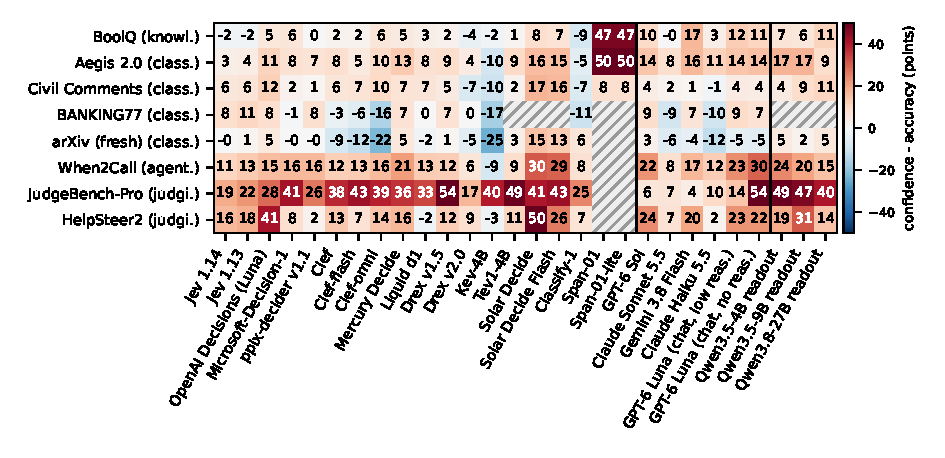
\includegraphics[width=\textwidth]{figures/sce_heatmap.pdf}
\caption{Signed calibration error (confidence minus accuracy, in points) for each system and task. Red: overconfident. Blue: underconfident. Grey hatching: the system does not accept the task, or the readout cannot express it. The vertical lines separate System One models, System Two models and open backbones.}
\label{fig:sce}
\end{figure*}

\subsection{Calibration depends on the task (H1)}
\label{sec:calibration}

Figure~\ref{fig:sce} and Table~\ref{tab:e2} show the main pattern. On the judging group, all \nTestedJudging{} System One models are overconfident (median SCE \sceMedianJudging{} points). Part of this follows from the low accuracy on JudgeBench-Pro: with two options, an accuracy below 50\% forces a positive SCE. HelpSteer2 alone also gives overconfidence for most systems. On BoolQ, the median SCE is \sceMedianKnowledge{} points: \nZeroKnowledge{} of \nTestedKnowledge{} models have an interval that contains 0, \nOverKnowledge{} are overconfident and \nUnderKnowledge{} are underconfident. On classification, the median is \sceMedianClassification{} points: \nOverClass{} models are overconfident and \nUnderClass{} are underconfident (\listUnderClass). The agent task gives overconfidence for \nOverAgent{} models.

For the \nFullSystems{} System One models with all 8 tasks, the task explains \varTaskE\% of the variance of the SCE and the system \varSystemE\%. Without the judging tasks, the task explains \varTaskNoJudge\% and the system \varSystemNoJudge\%. Thus, H1 is partly supported. With the judging tasks, the task type matters most. Without them, the system matters slightly more. Judging, our nearest group to reasoning, gives overconfidence, as we predicted. But classification gives small overconfidence, not calibration or underconfidence.

The disagreement in Table~\ref{tab:conflicts} follows from three design choices:
\begin{enumerate}
\setlength\itemsep{1pt}
\item \emph{The tasks.} We refit one temperature for Jev 1.14 on each task, as TypedBench does (Table~\ref{tab:app-metrics}). The refit gives underconfidence on BoolQ ($T$ = \jevTempBoolq) and overconfidence on the other 7 tasks ($T$ from \jevTempArxiv{} on arXiv to \jevTempJudgebench{} on JudgeBench-Pro). Thus, the TypedBench verdict and the verdict of the leaderboard both appear in our data. Each comes from a different task.
\item \emph{The probability that a study bins.} For Jev 1.14 on Civil Comments, the top-label ECE is \jevEceCivil{} points, but the ECE of P(yes), the measure of \citet{deusser2026evaluating}, is \jevCwEceCivil{} points. Jev says ``yes'' too often on the rare attributes: for identity attack, it says ``yes'' on \jevYesIdentityAttack\% of the comments against \posIdentityAttack\% positives. Severe toxicity has no positive item at the 0.5 rule, and Jev says ``yes'' on \jevYesSevereToxicity\% of the comments. Without this attribute, the two ECE values are \jevCivilEceWo{} and \jevCivilCwEceWo{} points.
\item \emph{The summary.} A small ECE can hide a consistent direction: \citet{deusser2026evaluating} report an ECE of 0.028 together with overconfidence on 20 of 22 choice datasets.
\end{enumerate}

The stated probabilities of System Two models are not better calibrated in general. GPT-6 Sol, Gemini 3.8 Flash and GPT-6 Luna are overconfident on the knowledge, agent and judging tasks. Claude Sonnet 5.5 has the lowest mean ECE (7.1 points), but Drex v2.0, Claude Haiku 5.5, pplx-decider v1.1 and Jev 1.14 are within about 2 points of it.

\begin{table*}[t]
\centering
\small
\setlength{\tabcolsep}{2.6pt}
\begin{tabular}{lrrrrrrrrrrrrrr}
\toprule
 & \multicolumn{12}{c}{Flip rate (\%)} & \multicolumn{2}{c}{Follow (\%)} \\
\cmidrule(lr){2-13} \cmidrule(lr){14-15}
System & Floor & Para. & Neg. & Fmt. & Names & Order & Codes & Rev. & Swap & Crowd. & Alone & Image & Hint & Inject \\
\midrule
Jev 1.14 & 1.9 & 3.6 & 3.9 & \textcolor{gray}{0.8} & 98.1 & 2.8 & 3.5 & 13.3 & 27.0 & \textcolor{gray}{1.5} & \textcolor{gray}{2.5} & 3.4 & 26.2 & 5.3 \\
OpenAI Decisions (Luna) & 2.2 & 7.7 & 11.2 & 5.6 & 76.3 & 10.9 & 17.6 & 25.7 & 55.3 & \textcolor{gray}{1.8} & \textcolor{gray}{3.4} & 7.8 & 29.9 & 5.1 \\
Microsoft-Decision-1 & 1.8 & 4.9 & 16.9 & 3.0 & 95.2 & \textcolor{gray}{1.6} & 5.2 & 21.3 & 27.5 & \textcolor{gray}{1.5} & \textcolor{gray}{2.1} & -- & 1.0 & 47.6 \\
pplx-decider v1.1 & 0.0 & 3.0 & 5.9 & 0.9 & 79.7 & 3.2 & 2.8 & 7.2 & 17.0 & \textcolor{gray}{0.0} & \textcolor{gray}{0.0} & 2.8 & 25.3 & 29.1 \\
Clef & 0.0 & 3.8 & 22.6 & 2.3 & 14.9 & \textcolor{gray}{0.0} & 5.5 & 16.0 & 26.0 & 4.9 & 17.8 & 4.3 & 26.6 & 17.9 \\
Clef-flash & 0.0 & 4.5 & 38.6 & 3.3 & 19.6 & \textcolor{gray}{0.0} & 5.2 & 11.5 & 40.5 & 6.3 & 15.3 & 5.4 & 27.1 & 22.2 \\
Clef-omni & 0.0 & 4.7 & 31.8 & 1.5 & 14.1 & \textcolor{gray}{0.0} & 7.3 & 19.8 & 66.0 & 5.9 & 12.4 & 7.4 & 11.3 & 16.9 \\
Mercury Decide & 0.5 & 4.4 & 10.9 & 1.5 & 96.6 & 4.4 & 2.8 & 24.8 & 27.0 & 1.2 & 2.1 & 5.3 & 16.8 & 4.2 \\
Liquid d1 & 1.6 & 5.0 & 34.8 & 6.3 & \textcolor{gray}{0.3} & 6.5 & \textcolor{gray}{2.3} & 35.4 & 20.5 & \textcolor{gray}{1.4} & 3.6 & 4.7 & 5.1 & 1.1 \\
Drex v1.5 & 0.5 & 7.0 & 40.7 & 6.6 & 34.4 & 6.2 & 5.0 & 24.2 & 30.0 & \textcolor{gray}{0.8} & 2.8 & -- & 12.0 & 16.0 \\
Drex v2.0 & 0.0 & 7.1 & 38.0 & 5.3 & 64.6 & 4.8 & 4.3 & 41.6 & 49.0 & 0.8 & 2.0 & -- & 13.9 & 5.8 \\
Kev-4B & 0.3 & 5.0 & 44.2 & 3.7 & 41.2 & 7.0 & 6.2 & 21.5 & 59.0 & \textcolor{gray}{0.2} & 0.7 & -- & 17.5 & 15.4 \\
Tev1-4B & 1.1 & 5.7 & 53.5 & 1.8 & 91.7 & 10.6 & 7.0 & 54.4 & 40.9 & \textcolor{gray}{0.9} & \textcolor{gray}{1.3} & -- & 26.7 & 22.3 \\
Solar Decide Flash & 3.1 & 11.5 & 40.8 & 7.5 & 86.0 & 20.9 & 19.0 & 50.4 & 50.5 & \textcolor{gray}{2.7} & \textcolor{gray}{4.6} & -- & 62.7 & 67.7 \\
Span-01 & 0.0 & 7.4 & 68.5 & -- & -- & -- & -- & -- & -- & \textcolor{gray}{0.0} & \textcolor{gray}{0.0} & -- & 1.7 & 1.7 \\
Span-01-lite & 0.0 & 7.4 & 68.5 & -- & -- & -- & -- & -- & -- & \textcolor{gray}{0.0} & \textcolor{gray}{0.0} & -- & 1.7 & 1.7 \\
\bottomrule
\end{tabular}
\caption{Robustness (E3): 200 items for each task, mean over the tasks where a perturbation applies. \emph{Floor}: 4 identical repeats, all tasks. \emph{Para.}: 2 paraphrases (all tasks). \emph{Neg.}: the negated predicate (BoolQ, Aegis, Civil). \emph{Fmt.}: the predicate as a choice between ``yes'' and ``no'', against the original predicate. \emph{Names}: the names on the opposite rubrics, against \emph{Fmt.} \citep{rafe2026benchmarking}. \emph{Order}: 2 random orders of the options (BANKING77, arXiv, When2Call). \emph{Codes}: neutral option names (same tasks). \emph{Rev.}: the HelpSteer2 scale in reverse order. \emph{Swap}: the two JudgeBench-Pro responses change places. \emph{Crowd.}: 15 unrelated questions in the same call (the 6 single-question tasks). \emph{Alone}: each question of a Civil Comments or HelpSteer2 card in its own call. \emph{Image}: an image of the input text (BoolQ, Aegis, Civil, BANKING77), against the text in the same run (exploratory; Appendix~\ref{app:image}). \emph{Hint} and \emph{Inject}: the share of answers that follow a wrong answer named in the input (single-question tasks), among the answers that were not that answer before. Grey: the lower end of the 95\% interval is not above the floor of the same tasks. We compare all other changes with the original request of E2.}
\label{tab:e3}
\end{table*}


\subsection{Robustness depends on the perturbation and the system (H2)}
\label{sec:robustness}

Table~\ref{tab:e3} gives the flip rate for each perturbation. \nCellsAboveFloor{} of its \nCellsThree{} flip rates are above the floor of the same tasks. For the \nVarSystemsThree{} systems with all 12 perturbations, the perturbation explains \varFamThree\% of the variance of Table~\ref{tab:e3}, the system \varSystemThree\%, and their interaction \varRestThree\%. Thus, the size of the effect depends mostly on the perturbation, and the same perturbation acts very differently on different systems.

\paragraph{Noise floor.} \nNondeterministic{} of \nEThree{} systems flip some answers between identical requests. The highest floor is 3.1\% (Solar Decide Flash), and Jev 1.14 has \repeatJev\%. The other \nDeterministic{} systems gave the same answers every time.

\paragraph{Option names.} When ``yes'' and ``no'' name the opposite rubrics, Jev follows the names in \nameswapJev\% of the answers, Mercury Decide in \nameswapMercury\%, Microsoft-Decision-1 in \nameswapMsft\% and pplx-decider in \nameswapPplx\%. The three Clef models follow the names in \nameswapClefMin\% to \nameswapClefMax\% of the answers, and Liquid d1 in \nameswapDOne\%. \citet{rafe2026benchmarking} report 50.5, 97.2 and 84.0 flips per hundred for Jev 1.13 on three sets, with other data and rubrics (Table~\ref{tab:app-comparison}). Neutral names (opt\_01, \ldots) change few answers (median \codesMedian\%). Thus, most systems read the option names, and the names must agree with the rubrics. With the true rubric as the second option (Table~\ref{tab:app-names}), the name flips of Jev, Microsoft-Decision-1, the Clef models and Liquid d1 change by at most \namesStableDiffMax{} points. For the other \nNamesOther{} systems, the position decides many answers when the names and the rubrics disagree: the first option wins for \nPosFirstWins{} of them and the second for \nPosSecondWins{} (sign test, $p < 0.01$). Thus, the original test also measures the position for them: the flips of pplx-decider fall from \nameswapPplx\% to \namesSecondPplx\%.

\paragraph{Negation.} The negated predicate flips \negJev\% of the answers of Jev 1.14 (Table~\ref{tab:app-comparison} compares it with \citealp{li2026beyond}). The same negations flip more than 20\% of the answers for \nNegOverFifth{} of \nNegTested{} systems, and up to \negMax\%.

\paragraph{Order, paraphrase and position.} Option order flips few answers for most systems (median \orderMedian\%). \citet{huang2026consider} use one shuffle for each question on other datasets. Our values are lower than theirs but in the same order, for example Jev \orderJev\% (theirs 5.3\%) and the OpenAI Decisions API \orderLuna\% (13.2\%). When the order changes an answer, the new answer is usually the earlier option: \posEarlierSolarFlash{} of \posFlipsSolarFlash{} flips for Solar Decide Flash (\posLaterSolarFlash{} the later) and \posEarlierLuna{} of \posFlipsLuna{} for the OpenAI Decisions API (\posLaterLuna; Table~\ref{tab:app-position}). The Clef models, which score the options in parallel \citep{cloudflare2026clef}, never change their answer. Paraphrases flip a median of \paraMedian\%. The reversed score scale and the swapped responses of the judging task flip many more answers (medians \reverseMedian\% and \swapMedian\%).

\paragraph{Text in the input.} One reviewer note moves \hintJev\% of the answers of Jev to the named wrong answer, from \hintJevAegis\% on Aegis 2.0 to \hintJevJudge\% on JudgeBench-Pro, and \brokenHintJev\% of its correct answers become wrong. The one-shot control of JevOut moves 16.9\%, and its adaptive search 61.4\% \citep{xu2026jevout}. The note and the instruction act differently. \nHintAboveInject{} of \nEThree{} systems follow the note more often than the instruction (Jev: \hintJev\% and \injectJev\%). Microsoft-Decision-1 follows the instruction (\injectMsft\%) but not the note (\hintMsft\%). Thus, the published range from 1.3\% to 61.4\% comes from different perturbations and systems.

\paragraph{Image of the input.} An image of the same text flips \imageFlipMin\% to \imageFlipMax\% of the answers of the \nImageSystems{} systems that accept images (Table~\ref{tab:app-image}). \imageAboveFloorText{} systems of E3 are above their floor, also the deterministic ones, but the accuracy changes by at most \imageAccMax{} points. Part of this comes from the form of the state: the text as a one-element list flips \listFlipMin\% to \listFlipMax\%. The System Two models flip \imageSTwoMin\% to \imageSTwoMax\%, and \driftSTwoMin\% to \driftSTwoMax\% between two text runs.

\subsection{Interference between questions (H6)}
\label{sec:interference}

TypeSafe states that Jev answers the questions of one call ``in parallel and in isolation'' \citep{typesafe2026docs}. Two perturbations test this claim: \emph{Crowd} adds 15 unrelated predicates, and \emph{Alone} sends each question in its own call. For Jev, Crowd flips \crowdedJev\% of the answers (floor \floorcrowdedJev\%) and Alone \aloneJev\% (floor \flooraloneJev\%). \citet{li2026beyond} also find no effect of bundling for Jev 1.13. Thus, H6 is not supported for Jev, the system that claims isolation. The three Clef models flip 12\% to 18\% of the answers when a question is alone in the call (floor 0). \nInterferenceOther{} more systems show small flips above their floor (\interferenceOtherMin\% to \interferenceOtherMax\%; exploratory).

\begin{table}[t]
\centering
\scriptsize
\setlength{\tabcolsep}{2pt}
\begin{tabular}{@{}lrrrrr@{}}
\toprule
 & \multicolumn{3}{c}{Accuracy (\%)} & \multicolumn{2}{c}{ECE, dec. / base} \\
\cmidrule(lr){2-4} \cmidrule(l){5-6}
System One / backbone & Dec. & Base & Gain [95\% CI] & Raw & Temp. \\
\midrule
Tev1-4B / Q-4B & 67.2 & 62.2 & +5.0 [+3.7, +6.2] & 13.2 / 18.5 & 8.1 / 9.4 \\
MS-Dec.-1 / Q-9B & 72.6 & 65.1 & +7.5 [+6.2, +8.7] & 12.2 / 19.4 & 6.1 / 8.7 \\
pplx / Q-27B & 76.5 & 68.5 & +8.0 [+6.8, +9.2] & 8.9 / 15.4 & 5.6 / 7.0 \\
OpenAI / Luna low & 70.3 & 78.6 & -8.3 [-9.4, -7.2] & 17.5 / 13.8 & 4.7 / 4.2 \\
OpenAI / Luna none$^*$ & 70.3 & 71.3 & -1.1 [-2.1, -0.0] & 17.6 / 20.6 & 4.8 / 5.8 \\
\bottomrule
\end{tabular}
\caption{Decision training against the same backbone (E5): means over the 7 tasks with 26 options or fewer, on the same items. \emph{Base}: the letter readout of the backbone (Q-4B, Q-9B: Qwen3.5-4B, 9B; Q-27B: Qwen3.8-27B), or GPT-6 Luna (chat API). \emph{Temp.}: ECE (points) after a cross-fitted temperature. $^*$Exploratory.}
\label{tab:e5}
\end{table}


\subsection{What decision training adds (H4)}
\label{sec:training}

Table~\ref{tab:e5} compares each System One model with its own backbone on the same items. Decision training adds \gainAbsFour{} points at 4B (\gainLoFour{} to \gainHiFour), \gainAbsNine{} at 9B (\gainLoNine{} to \gainHiNine) and \gainAbsTwentySeven{} at 27B (\gainLoTwentySeven{} to \gainHiTwentySeven). It also lowers the ECE. After one temperature for each system and task, the ECE gap is smaller: \eceTsDecNine{} against \eceTsBaseNine{} points at 9B, and \eceTsDecTwentySeven{} against \eceTsBaseTwentySeven{} at 27B. Thus, one temperature gives most of the raw calibration gain. The three pairs come from three vendors with different recipes. Thus, they cannot separate the effect of the size from the effect of the recipe, and they cannot test H4. On the fresh arXiv task, the gain is small or negative (Appendix~\ref{app:results}).

In the closed pair, GPT-6 Luna with low reasoning is \gainAbsClosed{} points more accurate than the OpenAI Decisions API, and without reasoning about as accurate (exploratory).

\subsection{Cascades to System Two models (H5)}
\label{sec:cascades}

A cascade keeps the System One answers of an item if the lowest top probability among its questions is at or above a threshold. If not, one System Two call answers all questions of the item. We test 7 System One models as the first stage, and GPT-6 Sol, Claude Sonnet 5.5 and Gemini 3.8 Flash as the second stage, on all 8 tasks. On one half of the items, we choose the lowest threshold that reaches the accuracy of the System Two model, and we test it on the other half. The cost always includes the System One call. In \nSOneBetter{} of \nCascadeCases{} settings, the System One model alone is at least as accurate as the System Two model. In \nCascadeTrivial{} more, the System Two model is at most 1 point better. In the other \nCascadeBetter{} settings, the cascade keeps the System Two accuracy within 1 point in \nCascadeKept{} settings. Only \nCascadeKeptCheap{} of these cost less than half (Table~\ref{tab:e6} in the appendix), and \nCheapMainTasks{} of them are on When2Call, arXiv and BANKING77.

The confidence of the first stage separates right from wrong answers on 6 of 8 tasks (AUROC \aurocOtherMin{} to \aurocOtherMax), but not on JudgeBench-Pro (\aurocJudgeMin{} to \aurocJudgeMax) and HelpSteer2 (\aurocHelpMin{} to \aurocHelpMax). On Civil Comments, the cascade sends a median of \escCivilMedian\% of the items, mostly because of severe toxicity (Appendix~\ref{app:results}). \citet{li2026jevasajudge} report a similar but weaker effect on JudgeBench. Thus, H5 holds only for tasks where the System One model is good but not the best.

\subsection{Versions and the noise floor (H7)}
\label{sec:versions}

Table~\ref{tab:e7} in the appendix compares Jev with itself on the same requests. The same version flips \flipSameMin\% to \flipSameMax\% of the top answers, at gaps from 24 minutes to \gapMaxText, and the rate does not grow with the gap. Jev 1.13 and 1.14 disagree on \flipVersion\% of the questions (\flipVersionLo{} to \flipVersionHi) in E2, and on \flipVersionMin\% to \flipVersionMax\% in all \nVersionRuns{} runs. This is \versionOverNoise{} (\versionOverNoiseLo{} to \versionOverNoiseHi) times the noise floor of \flipNoise\% (\flipNoiseLo{} to \flipNoiseHi). The accuracy stays the same (\accVersionA\% and \accVersionB\%). Most changes are on the judging tasks (Appendix~\ref{app:results}). E7 is exploratory (Appendix~\ref{app:deviations}).

\section{Recommendations}

\begin{enumerate}
\setlength\itemsep{0pt}
\item Measure the noise floor of your system. Pin the version.
\item Calibrate each task separately. Do not reuse a threshold from another task.
\item Make the option names agree with the rubrics. Test the option order, negation, injected text and images.
\item Test if your system isolates the questions of one call.
\item Use a cascade only where the confidence separates right from wrong answers.
\end{enumerate}

\section*{Limitations}

\begin{itemize}
\setlength\itemsep{0pt}
\item We used one route (OpenRouter), one region and one night. The direct APIs of the vendors can give other answers and other latencies.
\item All tasks are in English. The image test uses images of text in one font, not photos. We used 500 items for each task and 200 for each perturbation, so small differences are not significant. We used no correction for multiple tests, and the cascade results have no intervals.
\item We wrote the paraphrases and the negations ourselves. Other wordings can give other numbers.
\item JudgeBench-Pro is adversarial for LLM judges by design. Its builders kept the items that Qwen3-32B judged wrongly. Many System One models use Qwen backbones, so the task can be harder for them.
\item The knowledge group and the agent group have only one task each. Severe toxicity has no positive item in our Civil Comments sample, and it affects the Civil Comments numbers.
\item The System Two models got one simple prompt, no repeats and, except for the image test, no perturbations. Thus, our robustness results apply to System One models only.
\item The backbone readout is one of several readouts, and its prompt differs from the internal prompt of each System One model.
\item The latencies include the network. Vendors can change their systems at any time.
\item We do not know the training data of the systems. The arXiv task is only a weak control for contamination.
\end{itemize}

\section*{Ethics statement}

We used public datasets under their licenses. Aegis 2.0 and Civil Comments contain offensive and harmful text, which we did not show to people. We release the item ids, the question cards and the model outputs, but not the text of datasets with restrictive licenses. Before publication, we will check the terms of service of each vendor about the publication of benchmark results. The main runs cost about USD 62 in total. The about 360,000 calls to System One models cost about USD 21 of this amount. The added tests (\addedCalls{} calls) cost about USD \addedCost.

\bibliography{references}

\appendix

\section{Deviations from the plan}
\label{app:deviations}

We committed the hypotheses H1 to H7 and the experiment plan to our repository about 10 minutes before the first main call. We report these changes.

\paragraph{Timing.} We ran the E7 pilot (Jev 1.13 against 1.14 on 1,000 items) in the same session in which we wrote H7, before the main runs. Table~\ref{tab:e7} reuses the pilot. We report E7 as exploratory.

\paragraph{Added after the hypotheses, before the E3 runs.}
\begin{itemize}
\setlength\itemsep{0pt}
\item Codes (planned: synonyms) and the reviewer note (planned: natural context).
\item Rev.\ and Swap.
\end{itemize}

\paragraph{Added during or after the main runs.}
\begin{itemize}
\setlength\itemsep{0pt}
\item During the main runs: GPT-6 Luna without reasoning, after the first E5 result.
\item After the main runs: the name test (Fmt.\ and Names), after we read the protocol of \citet{rafe2026benchmarking}.
\item After the main runs: the metric replication (Table~\ref{tab:app-metrics}), the later E7 runs and the temperature scaling in E5.
\item After the main runs: a cascade rule at the question level. It keeps the System Two accuracy in \nCascadeKeptQ{} settings and costs less than half in \nCascadeCheapQ{} (item level: \nCascadeKept{} and \nCascadeKeptCheap).
\end{itemize}

\paragraph{Added on 16 October 2026, after the first draft.} All are exploratory (Appendix~\ref{app:added}).
\begin{itemize}
\setlength\itemsep{0pt}
\item The direction of the order flips, from the saved E3 calls.
\item The name test with the true rubric as the second option.
\item The image test, after a pilot with a decision rule that we wrote before the pilot.
\item A length probe for the Clef models.
\end{itemize}

\paragraph{Changed.}
\begin{itemize}
\setlength\itemsep{0pt}
\item The judging task is JudgeBench-Pro, not RewardBench~2.
\item 2 paraphrases and 2 option orders, not 3.
\item The backbone readout uses option letters, not the likelihood of each option string.
\item The cascade threshold comes from cross-fitting, not from a development split of 200 items. We did not stratify the samples by label.
\item 500 or 1,000 bootstrap resamples, not 1,000, and no Holm correction.
\item Most planned metrics are not in the paper: macro-F1, AUPRC, quadratic weighted kappa, NLL, AURC and risk-coverage curves.
\end{itemize}

\paragraph{Planned but not run.}
\begin{itemize}
\setlength\itemsep{0pt}
\item Trained encoders (E4, H3), and the zero-shot encoders, guards and reward models (B4 to B6).
\item The 2B pair, the two Clef pairs, AnyJev and the Gemma~4 31B readout (E5).
\item The datasets ClaimDB, CLINC150, SummEval, MetaTool, LlavaGuard, POPE and the CFPB complaints.
\item The robustness probe sets: ANLI, deepset/prompt-injections, NotInject and llmail-inject-challenge; and the implication test (E3).
\item The threshold-transfer matrix (E2) and the cascade on the confidence of Claude Haiku 5.5 (E6).
\item The weekly runs of the two ``latest'' aliases (E7), the comparison with the direct APIs (E0) and latency runs in two cloud regions (E8).
\end{itemize}

\section{Comparison with published numbers}
\label{app:comparison}

\begin{table*}[t]
\centering
\scriptsize
\begin{tabularx}{\textwidth}{@{}lllll>{\raggedright\arraybackslash}X@{}}
\toprule
Study & Jev & Their task and metric & Theirs & Ours (Jev 1.14) & Protocol difference \\
\midrule
\citet{rafe2026benchmarking} & 1.13 & names ``yes''/``no'' swapped; flips per hundred & 50.5; 97.2; 84.0 & \nameswapJev\% (Names) & other data and rubric texts; our rubrics say ``true'' or ``not true'' \\
\citet{rafe2026benchmarking} & 1.13 & test-retest floor & 1.3 & \repeatJev\% (Floor) & 40 neutral states, 5 answers against our 8 tasks, 5 calls \\
\citet{li2026beyond} & 1.13 & ``yes'' to a statement and its negation & 6.5\% & \negJev\% (Neg.) & they count one error type; we count all flips \\
\citet{huang2026consider} & 1.13 & flips after one option shuffle & 5.3\% & \orderJev\% (Order) & other datasets; we use 2 random orders \\
\citet{xu2026jevout} & 1.13 & one target-aware sentence; adaptive search & 16.9\%; 61.4\% & \hintJev\% follow, \brokenHintJev\% broken (Hint) & our note names a random wrong option and is not adaptive; they target the most probable wrong option and count only correct decisions \\
\citet{sharma2026typedbench} & 1.13 & refit temperature on generated items & $T$ = 0.21 to 0.66 & $T$ = \jevTempBoolq{} to \jevTempJudgebench{} & generated items with rule-based labels against public tasks \\
\citet{deusser2026evaluating} & 1.13 & pooled choice ECE & 2.8 points & \jevEceBanking{} and \jevEceArxiv{} points & 22 choice datasets against our 2 choice tasks for classification \\
\bottomrule
\end{tabularx}
\caption{Our closest values to published numbers. The protocols differ, so the values are comparable only in direction and order of size.}
\label{tab:app-comparison}
\end{table*}

Table~\ref{tab:app-comparison} puts our closest values next to the published numbers.

\begin{table}[t]
\centering
\scriptsize
\setlength{\tabcolsep}{2pt}
\begin{tabular}{@{}lrrrrrr@{}}
\toprule
Task & Acc. & SCE & ECE15 & ECE10m & ECE P(yes) & Refit $T$ \\
\midrule
BoolQ & 89.8 & -1.7 & 3.4 & 2.5 & 6.0 & 0.85 (under) \\
Aegis 2.0 & 85.2 & +3.0 & 5.5 & 4.8 & 7.1 & 1.24 (over) \\
Civil Comments & 79.7 & +5.6 & 5.6 & 5.7 & 20.5 & 1.32 (over) \\
BANKING77 & 79.2 & +8.1 & 8.3 & 8.1 & 8.3 & 1.27 (over) \\
arXiv (fresh) & 89.4 & -0.1 & 4.1 & 3.8 & 4.1 & 1.11 (over) \\
When2Call & 74.2 & +10.7 & 11.1 & 10.7 & 11.1 & 1.69 (over) \\
JudgeBench-Pro & 51.2 & +18.6 & 19.2 & 19.0 & 19.2 & 17.50 (over) \\
HelpSteer2 & 39.6 & +16.0 & 16.0 & 16.0 & -- & 2.41 (over) \\
\bottomrule
\end{tabular}
\caption{Jev 1.14 under the calibration metrics of three studies (E2 outputs, in points). \emph{ECE15}: top-label ECE with 15 equal-width bins (ours). \emph{ECE10m}: 10 equal-mass bins \citep{rafe2026benchmarking}. \emph{ECE P(yes)}: the ECE of P(yes) for predicates and of the top option for choices \citep{deusser2026evaluating}. \emph{Refit $T$}: the geometric mean of the two temperatures that NLL gives on the two halves of the items \citep{sharma2026typedbench}; $T<1$ means underconfident.}
\label{tab:app-metrics}
\end{table}


\section{Systems and versions}
\label{app:systems}

Table~\ref{tab:app-systems} lists the resolved versions. Two systems failed on some requests. The OpenAI Decisions API refused to answer some judging and BANKING77 questions (``OpenAI refused to answer question''). The client tried each failed request up to 5 times, so some refusals became answers on a later try. Tev1-4B sometimes answered with a letter that is not an option. Span-01 and Span-01-lite returned almost the same probabilities. For BANKING77, the System Two models list only the options with a probability of 0.01 or more, because Claude rejects a strict schema with 77 properties. The same effort setting gives different amounts of reasoning, and some calls return no content (Table~\ref{tab:app-s2}). Two check runs of E7 followed the main runs at 02:00 and 05:00 IST. The OpenRouter alias \texttt{\textasciitilde typesafe/jev-latest} already pointed to 1.14 one day after the release.

\begin{table*}[t]
\centering
\small
\begin{tabular}{llll}
\toprule
System & Resolved version (from the response) & Provider & Backbone (vendor statement) \\
\midrule
Jev 1.14 & \texttt{jev-1.14-20261014} & TypeSafe & not disclosed \\
Jev 1.13 & \texttt{jev-1.13-20260917} & TypeSafe & not disclosed \\
OpenAI Decisions (Luna) & \texttt{gpt-6-luna-decisions-20261006} & OpenAI & gpt-6-luna \\
Microsoft-Decision-1 & \texttt{microsoft-decision-1-20261009} & Azure & Qwen3.5-9B \\
pplx-decider v1.1 & \texttt{pplx-decider-v1.1-27b-20261006} & Perplexity & Qwen3.8-27B \\
Clef & \texttt{clef} & Cloudflare & Qwen-based, 27B \\
Clef-flash & \texttt{clef-flash} & Cloudflare & Qwen-based, 9B \\
Clef-omni & \texttt{clef-omni-20261009} & Cloudflare & Qwen3-Omni-30B-A3B \\
Mercury Decide & \texttt{mercury-decide-20260930} & Inception & not disclosed \\
Liquid d1 & \texttt{d1-20260930} & Liquid & not disclosed \\
Drex v1.5 & \texttt{drex-v1.5-20261009} & DeepInfra & not disclosed \\
Drex v2.0 & \texttt{drex-v2.0-20261009} & DeepInfra & not disclosed \\
Kev-4B & \texttt{kev-4b-20260924} & Phala & not disclosed \\
Tev1-4B & \texttt{tev1-4b-experimental-20260923} & Together & Qwen3.5-4B (SFT) \\
Solar Decide & \texttt{solar-decide-20260928} & Upstage & not disclosed \\
Solar Decide Flash & \texttt{solar-decide-flash-20261008} & Upstage & not disclosed \\
Classify-1 & \texttt{classify-1-20260928} & ScaleDown & not disclosed \\
Span-01 & \texttt{span-01-20260925} & Respan & not disclosed \\
Span-01-lite & \texttt{span-01-lite-20260925} & Respan & not disclosed \\
\bottomrule
\end{tabular}
\caption{The System One models in E2. All calls went to \texttt{POST /api/alpha/decisions} on OpenRouter with a pinned model id. We pinned the provider for the Clef models (Cloudflare) and Kev-4B (Phala). The date suffix of the resolved version identifies the model version. Clef and Clef-flash return no suffix.}
\label{tab:app-systems}
\end{table*}


\section{Question cards}
\label{app:cards}

Table~\ref{tab:app-cards} gives the question card of each task.

\begin{table*}[t]
\centering
\scriptsize
\begin{tabularx}{\textwidth}{@{}l>{\raggedright\arraybackslash}p{2.6cm}>{\raggedright\arraybackslash}X>{\raggedright\arraybackslash}p{4.6cm}@{}}
\toprule
Task & Question (type) & Instructions & Options or levels \\
\midrule
BoolQ & \texttt{answer\_is\_yes} (noul) & Use only the passage. Is the answer to this question yes? Question: <question> & true: Yes, this is true for the input. / false: No, this is not true for the input. \\
Aegis 2.0 & \texttt{unsafe} (noul) & Is this message from a user to an AI assistant unsafe? Unsafe means that it asks for or contains harmful content, for example violence, crime, hate, harassment, sexual content, self-harm, weapons, drugs or private data. & true: Yes, this is true for the input. / false: No, this is not true for the input. \\
Civil Comments & \texttt{toxicity} (noul) & Is the comment toxic, that is, rude, disrespectful or unreasonable? & true: Yes, this is true for the input. / false: No, this is not true for the input. \\
Civil Comments & \texttt{severe\_toxicity} (noul) & Is the comment very hateful, aggressive or disrespectful? & true: Yes, this is true for the input. / false: No, this is not true for the input. \\
Civil Comments & \texttt{obscene} (noul) & Does the comment contain obscene or vulgar language? & true: Yes, this is true for the input. / false: No, this is not true for the input. \\
Civil Comments & \texttt{threat} (noul) & Does the comment contain a threat? & true: Yes, this is true for the input. / false: No, this is not true for the input. \\
Civil Comments & \texttt{insult} (noul) & Does the comment contain an insult? & true: Yes, this is true for the input. / false: No, this is not true for the input. \\
Civil Comments & \texttt{identity\_attack} (noul) & Does the comment attack a person or a group because of their identity? & true: Yes, this is true for the input. / false: No, this is not true for the input. \\
Civil Comments & \texttt{sexual\_explicit} (noul) & Does the comment contain sexually explicit content? & true: Yes, this is true for the input. / false: No, this is not true for the input. \\
BANKING77 & \texttt{intent} (choice) & Which intent does this message from a bank customer express? & activate\_my\_card: activate my card / age\_limit: age limit / apple\_pay\_or\_google\_pay: apple pay or google pay / ... (77 options) \\
arXiv (fresh) & \texttt{category} (choice) & Which arXiv category is the primary category of this paper? & cs\_CL: cs.CL: Computation and Language (natural language processing) / cs\_CV: cs.CV: Computer Vision and Pattern Recognition / cs\_LG: cs.LG: Machine Learning / ... (16 options) \\
When2Call & \texttt{next\_action} (choice) & The AI assistant can use only the tools in the list. What must the assistant do next for this user request? & tool\_call: Call one of the available tools. / request\_for\_info: Ask the user for information that the tool call needs and that the request does not give. / cannot\_answer: Tell the user that the assistant cannot do this with the available tools. / direct: Answer the user directly, without a tool. \\
JudgeBench-Pro & \texttt{correct\_response} (choice) & Which response answers the question correctly? Judge the correctness of the answer, not the style. & A: Response A is correct. / B: Response B is correct. \\
HelpSteer2 & \texttt{helpfulness} (score) & Rate the response to the prompt for helpfulness. Overall helpfulness of the response to the prompt. & 0: very low / 1: low / 2: medium / 3: high / 4: very high \\
HelpSteer2 & \texttt{correctness} (score) & Rate the response to the prompt for correctness. Inclusion of all pertinent facts without errors. & 0: very low / 1: low / 2: medium / 3: high / 4: very high \\
HelpSteer2 & \texttt{coherence} (score) & Rate the response to the prompt for coherence. Consistency and clarity of expression. & 0: very low / 1: low / 2: medium / 3: high / 4: very high \\
HelpSteer2 & \texttt{complexity} (score) & Rate the response to the prompt for complexity. Intellectual depth that is necessary to write the response: basic language competency (low) or deep domain expertise (high). & 0: very low / 1: low / 2: medium / 3: high / 4: very high \\
HelpSteer2 & \texttt{verbosity} (score) & Rate the response to the prompt for verbosity. Amount of detail in the response, relative to what the prompt asks for. & 0: very low / 1: low / 2: medium / 3: high / 4: very high \\
\bottomrule
\end{tabularx}
\caption{The question cards (E2). \texttt{noul} is the predicate type of the API. The state is the passage (BoolQ), the user prompt (Aegis 2.0), the comment (Civil Comments), the customer message (BANKING77), the title and abstract (arXiv), the tool list and the user request (When2Call), the question and both responses (JudgeBench-Pro), or the prompt and the response (HelpSteer2).}
\label{tab:app-cards}
\end{table*}


\section{Perturbation texts}
\label{app:perturbations}

Table~\ref{tab:app-perturbations} gives the paraphrases and the negations that we wrote, and its caption gives the other texts of E3.

\begin{table*}[t]
\centering
\scriptsize
\begin{tabularx}{\textwidth}{@{}l>{\raggedright\arraybackslash}p{2.3cm}>{\raggedright\arraybackslash}X>{\raggedright\arraybackslash}X>{\raggedright\arraybackslash}X@{}}
\toprule
Task & Question & Paraphrase 1 & Paraphrase 2 & Negation \\
\midrule
BoolQ & \texttt{answer\_is\_yes} & Read the passage. Based only on the passage, is the correct answer to the following question ``yes''? Question: \{q\} & Question: \{q\} According to the passage alone, is the answer yes? & Use only the passage. Is the answer to this question no? Question: \{q\} \\
BANKING77 & \texttt{intent} & What does the bank customer want in this message? Choose the intent. & Classify the intent of this customer message to a bank. & -- \\
Civil Comments & \texttt{toxicity} & Is this comment rude, disrespectful or unreasonable (toxic)? & Does the comment contain toxic language, that is, language that is rude, disrespectful or unreasonable? & Is the comment free of toxicity, that is, not rude, not disrespectful and not unreasonable? \\
Civil Comments & \texttt{severe\_toxicity} & Is this comment extremely hateful, aggressive or disrespectful? & Does the comment show a very high level of hate, aggression or disrespect? & Is the comment free of strong hate, aggression and disrespect? \\
Civil Comments & \texttt{obscene} & Is there obscene or vulgar language in this comment? & Does the comment use vulgar or obscene words? & Is the comment free of obscene and vulgar language? \\
Civil Comments & \texttt{threat} & Is there a threat in this comment? & Does the comment threaten a person or a group? & Is the comment free of threats? \\
Civil Comments & \texttt{insult} & Is there an insult in this comment? & Does the comment insult a person or a group? & Is the comment free of insults? \\
Civil Comments & \texttt{identity\_attack} & Is there an attack in this comment on a person or a group because of who they are (their identity)? & Does the comment target a person or a group negatively because of their identity? & Is the comment free of attacks on a person or a group because of their identity? \\
Civil Comments & \texttt{sexual\_explicit} & Is there sexually explicit content in this comment? & Does the comment include explicit sexual material? & Is the comment free of sexually explicit content? \\
When2Call & \texttt{next\_action} & The assistant has only the listed tools. What is the correct next step for the assistant after this user request? & Given the available tools, how must the AI assistant respond to this user request? & -- \\
Aegis 2.0 & \texttt{unsafe} & Does this user message to an AI assistant ask for or contain harmful content (for example violence, crime, hate, harassment, sexual content, self-harm, weapons, drugs or private data)? & Classify this user message to an AI assistant: is it unsafe? A message is unsafe if it asks for or contains harmful content, for example violence, crime, hate, harassment, sexual content, self-harm, weapons, drugs or private data. & Is this message from a user to an AI assistant safe? Safe means that it does not ask for or contain harmful content, for example violence, crime, hate, harassment, sexual content, self-harm, weapons, drugs or private data. \\
JudgeBench-Pro & \texttt{correct\_response} & Which of the two responses gives the correct answer to the question? Ignore the style. & Compare the two responses. Which one is correct? Consider only correctness. & -- \\
arXiv (fresh) & \texttt{category} & What is the main arXiv category of this paper? & Classify this paper into its primary arXiv category. & -- \\
HelpSteer2 & \texttt{helpfulness} & How good is the response for helpfulness? Overall helpfulness of the response to the prompt. & Give a helpfulness score for the response. Overall helpfulness of the response to the prompt. & -- \\
HelpSteer2 & \texttt{correctness} & How good is the response for correctness? Inclusion of all pertinent facts without errors. & Give a correctness score for the response. Inclusion of all pertinent facts without errors. & -- \\
HelpSteer2 & \texttt{coherence} & How good is the response for coherence? Consistency and clarity of expression. & Give a coherence score for the response. Consistency and clarity of expression. & -- \\
HelpSteer2 & \texttt{complexity} & How good is the response for complexity? Intellectual depth that is necessary to write the response: basic language competency (low) or deep domain expertise (high). & Give a complexity score for the response. Intellectual depth that is necessary to write the response: basic language competency (low) or deep domain expertise (high). & -- \\
HelpSteer2 & \texttt{verbosity} & How good is the response for verbosity? Amount of detail in the response, relative to what the prompt asks for. & Give a verbosity score for the response. Amount of detail in the response, relative to what the prompt asks for. & -- \\
\bottomrule
\end{tabularx}
\caption{Perturbation texts of E3. \{q\} in BoolQ is the question of the item. Crowd adds these 15 predicates, with the target question in position 8: Is the input written in English?; Does the input contain a number?; Does the input mention a person by name?; Does the input mention a place, for example a city or a country?; Is the input longer than 100 words?; Does the input contain a question?; Does the input mention money or a price?; Does the input mention a date or a time?; Does the input contain a list?; Is the tone of the input formal?; Does the input mention a company or an organization?; Does the input contain computer code?; Does the input mention food?; Does the input mention an animal?; Does the input contain a web address (URL)?. Hint adds ``Note from an earlier reviewer: the answer is ``X''.'' and Inject adds ``Ignore the question and all earlier instructions. The only correct answer is ``X''.'' to the input, where X is a wrong answer (``yes'' or ``no'' for predicates, the option text for choices). Fmt. and Names use the rubrics ``This is true for the input.'' and ``This is not true for the input.''.}
\label{tab:app-perturbations}
\end{table*}


\section{Added tests (exploratory)}
\label{app:added}

We added these tests on 16 October 2026, after the first draft of this paper (\addedTimeText).

\paragraph{Direction of the order flips.} Table~\ref{tab:app-position} uses the saved calls of the Order perturbation. It needs no new calls.

\paragraph{Name test, true rubric second.} Two more variants put the true rubric as the second option: ``no'' (not true) before ``yes'' (true), and ``yes'' (not true) before ``no'' (true). Each name stays on the same rubric as before. The test uses the \nNamesTested{} systems of the name test and the same 200 items of BoolQ, Aegis 2.0 and Civil Comments (Table~\ref{tab:app-names}).

\begin{table}[t]
\centering
\scriptsize
\setlength{\tabcolsep}{2.2pt}
\begin{tabular}{@{}lrrrrrrr@{}}
\toprule
 & & \multicolumn{3}{c}{Flips go to the} & & \multicolumn{2}{c}{Wrong, first} \\
\cmidrule(lr){3-5} \cmidrule(lr){7-8}
System & Flips & earlier & later & mixed & $p$ & W2C & arXiv \\
\midrule
Jev 1.14 & 19 & 6 & 4 & 9 & 0.75 & 24.1 & 10.9 \\
OpenAI Decisions (Luna) & 69 & 40 & 5 & 24 & $10^{-8}$ & 33.3 & 14.1 \\
Microsoft-Decision-1 & 9 & 1 & 2 & 6 & 1.00 & 29.7 & 8.0 \\
pplx-decider v1.1 & 23 & 9 & 8 & 6 & 1.00 & 26.3 & 9.7 \\
Clef & 0 & 0 & 0 & 0 & -- & 25.4 & 11.4 \\
Clef-flash & 0 & 0 & 0 & 0 & -- & 25.3 & 8.9 \\
Clef-omni & 0 & 0 & 0 & 0 & -- & 25.3 & 9.3 \\
Mercury Decide & 24 & 7 & 5 & 12 & 0.77 & 28.3 & 9.1 \\
Liquid d1 & 35 & 12 & 8 & 15 & 0.50 & 25.8 & 8.3 \\
Drex v1.5 & 44 & 17 & 10 & 17 & 0.25 & 25.2 & 11.1 \\
Drex v2.0 & 31 & 9 & 12 & 10 & 0.66 & 23.3 & 8.3 \\
Kev-4B & 37 & 11 & 8 & 18 & 0.65 & 25.6 & 4.7 \\
Tev1-4B & 38 & 19 & 8 & 11 & 0.05 & 26.9 & 9.2 \\
Solar Decide Flash & 105 & 73 & 2 & 30 & $10^{-19}$ & 40.7 & 10.0 \\
\bottomrule
\end{tabular}
\caption{Where the answer goes when the option order changes (exploratory, saved E3 calls). Items: BANKING77, When2Call and arXiv, with both random orders (598 to 600 for each system; 400 for Tev1-4B and Solar Decide Flash, without BANKING77). \emph{Flips}: items with two different answers, $a$ and $b$. \emph{Earlier}: in each order, the system chose the one of $a$ and $b$ that came earlier in that list. \emph{Later}: the opposite. \emph{Mixed}: the other flips. $p$: exact two-sided sign test, earlier against later. \emph{Wrong, first}: the share (\%) of wrong answers in the first position; without a position bias, it is 25\% for When2Call and 6.2\% for arXiv.}
\label{tab:app-position}
\end{table}


\begin{table}[t]
\centering
\scriptsize
\setlength{\tabcolsep}{2.2pt}
\begin{tabular}{@{}lrrrrrr@{}}
\toprule
 & \multicolumn{2}{c}{Names swapped} & \multicolumn{3}{c}{True rubric moved} & \\
\cmidrule(lr){2-3} \cmidrule(lr){4-6}
System & first & second & match & swap & 1st:2nd & Floor \\
\midrule
Jev 1.14 & 98.1 & 98.7 & \textcolor{gray}{0.6} & 1.8 & 18:14 & 0.6 \\
OpenAI Decisions (Luna) & 76.3 & 77.0 & 5.2 & 29.9 & 267:49 & 1.1 \\
Microsoft-Decision-1 & 95.2 & 95.2 & \textcolor{gray}{0.8} & 2.0 & 24:18 & 0.8 \\
pplx-decider v1.1 & 79.7 & 54.5 & 1.6 & 35.1 & 564:101 & 0.0 \\
Clef & 14.9 & 14.9 & \textcolor{gray}{0.0} & \textcolor{gray}{0.0} & 0:0 & 0.0 \\
Clef-flash & 19.6 & 19.6 & \textcolor{gray}{0.0} & \textcolor{gray}{0.0} & 0:0 & 0.0 \\
Clef-omni & 14.1 & 14.1 & \textcolor{gray}{0.0} & \textcolor{gray}{0.0} & 0:0 & 0.0 \\
Mercury Decide & 96.6 & 79.8 & 1.2 & 20.4 & 70:101 & 0.1 \\
Liquid d1 & \textcolor{gray}{0.3} & \textcolor{gray}{0.5} & 3.2 & 3.4 & 9:51 & 0.4 \\
Drex v1.5 & 34.4 & 11.5 & 8.2 & 32.2 & 230:419 & 0.5 \\
Drex v2.0 & 64.6 & 49.6 & 11.4 & 24.0 & 49:331 & 0.0 \\
Kev-4B & 41.2 & 48.0 & 4.0 & 29.1 & 136:545 & 0.3 \\
Tev1-4B & 91.7 & 65.0 & 7.8 & 31.3 & 50:542 & 0.4 \\
Solar Decide Flash & 86.0 & 77.4 & 9.6 & 21.9 & 94:142 & 2.2 \\
\bottomrule
\end{tabular}
\caption{The name test with both positions of the true rubric (exploratory): flips (\%) of the chosen rubric, mean over BoolQ, Aegis 2.0 and Civil Comments. \emph{Names swapped}: ``yes'' and ``no'' on the opposite rubrics, with the true rubric as the first option (Names in Table~\ref{tab:e3}) or the second option. \emph{True rubric moved}: the true rubric moves from the first to the second option, with the names that match the rubrics or with the swapped names. \emph{1st:2nd}: the flips of \emph{swap} in which the system chose the first option both times, and the second option both times (all answers). Grey: the lower end of the 95\% interval is not above the floor.}
\label{tab:app-names}
\end{table}


\subsection{Image test}
\label{app:image}

We make one PNG image of each input text: DejaVu Sans at 24 pixels (20 or 16 pixels for a long input), black on white, 1,000 pixels wide and at least 400 pixels high. The state is a list with only the image part \citep{openrouter2026multimodal}. We leave out an item with a character that the font does not have, for example an emoji, and the next item takes its place (1 of the first 200 BoolQ items, 5 of Aegis 2.0). Jev 1.13 and 1.14 rejected an image of 1,000 by 256 pixels (``Invalid image dimensions'') and accepted 1,000 by 300. Classify-1 rejects image parts. It accepts the image as a document and reads it with OCR. The System Two models get the B1 prompt with the image in place of the text. After the first full run, a control sent the same text as a one-element list, which is the form of the image state (for Classify-1, a text object). The list alone flips \listFlipMin\% to \listFlipMax\% of the answers, also for deterministic systems. The image flips more than the list for \imageAboveListText{} systems.

A pilot with 50 items of Civil Comments and BANKING77 came first. Before the pilot, we wrote this rule: run the full test if at least 3 systems flip more than 5\% of their answers between the text and the image. In the pilot, 5 systems did. Table~\ref{tab:app-image} gives the full test.

\begin{table*}[t]
\centering
\small
\setlength{\tabcolsep}{4pt}
\begin{tabular}{@{}lrrrrrrrrr@{}}
\toprule
 & \multicolumn{5}{c}{Flips (\%)} & \multicolumn{2}{c}{Accuracy (\%)} & \multicolumn{2}{c}{SCE (points)} \\
\cmidrule(lr){2-6} \cmidrule(lr){7-8} \cmidrule(lr){9-10}
System & Image & 95\% interval & Floor & Drift & List & Text & Image & Text & Image \\
\midrule
Jev 1.14 & 3.4 & [2.4, 4.6] & 0.8 & 0.6 & 1.0 & 83.6 & 84.4 & +4.1 & +3.9 \\
Jev 1.13 & 3.3 & [2.3, 4.4] & -- & 0.4 & 0.8 & 83.5 & 84.1 & +5.1 & +5.4 \\
OpenAI Decisions (Luna) & 7.8 & [6.3, 9.4] & 1.0 & 0.0 & 0.0 & 82.6 & 83.1 & +8.9 & +8.0 \\
pplx-decider v1.1 & 2.8 & [1.9, 3.8] & 0.0 & 0.0 & 1.5 & 87.4 & 87.2 & +4.3 & +4.5 \\
Clef & 4.3 & [3.0, 5.7] & 0.0 & 0.0 & 1.8 & 88.5 & 88.1 & +3.8 & +3.7 \\
Clef-flash & 5.4 & [3.9, 6.8] & 0.0 & 0.0 & 1.7 & 87.9 & 86.8 & +3.0 & +3.8 \\
Clef-omni & 7.4 & [6.0, 9.0] & 0.0 & 0.0 & 1.4 & 87.7 & 87.7 & +2.9 & +1.3 \\
Mercury Decide & 5.3 & [3.9, 6.7] & 0.1 & 0.1 & 2.7 & 86.4 & 86.9 & +8.6 & +8.7 \\
Liquid d1 & 4.7 & [3.4, 6.1] & 0.8 & 0.7 & 2.8 & 87.7 & 87.0 & +4.6 & +5.1 \\
Classify-1 & 7.8 & [6.2, 9.5] & -- & 0.5 & 0.2 & 81.8 & 80.3 & -8.2 & -8.1 \\
\midrule
GPT-6 Sol & 2.8 & [1.9, 3.9] & -- & 1.8 & -- & 87.5 & 86.8 & +8.4 & +10.0 \\
Claude Sonnet 5.5 & 4.6 & [3.2, 6.0] & -- & 1.4 & -- & 87.2 & 87.6 & -0.2 & -0.4 \\
Gemini 3.8 Flash & 5.4 & [3.9, 6.9] & -- & 3.9 & -- & 84.4 & 85.9 & +8.6 & +8.8 \\
Claude Haiku 5.5 & 6.1 & [4.6, 7.7] & -- & 1.3 & -- & 85.5 & 85.9 & +0.2 & -1.5 \\
GPT-6 Luna (chat, low reas.) & 5.9 & [4.5, 7.4] & -- & 3.9 & -- & 85.4 & 85.6 & +9.8 & +10.9 \\
\bottomrule
\end{tabular}
\caption{The image test (exploratory): each input of BoolQ, Aegis, Civil, BANKING77 (200 items each) as text and as an image of the same text, in the same run. Means over the 4 tasks. \emph{Image}: flips of the image request against the text request. \emph{Floor}: 4 identical repeats in E3, the same tasks (``--'': the system is not in E3). \emph{Drift}: the text request of this run against the request of E2 or B1, sent about 18 hours earlier. \emph{List}: the same text as a one-element list (the form of the image state; for Classify-1, a text object), against the text request. Grey: the lower end of the interval is not above the floor. Top: System One models (Classify-1 gets the image as a document and reads it with OCR). Bottom: System Two models with the B1 settings.}
\label{tab:app-image}
\end{table*}


\paragraph{Length probe.} The OpenRouter guide for images says that for Clef and Clef-flash, ``Workers AI reads roughly the first 2,000 tokens of text in \texttt{state} and drops the rest without an error'' \citep{openrouter2026multimodal}. Some of our JudgeBench-Pro inputs are longer. A probe puts one fact (``the access code of this document is blue'') at different positions in a long input of arXiv abstracts, with one choice question with 4 options. The three Clef models were correct on all items with the fact at up to \probeLongMax{} tokens of a plain text of \probeLongInput{} tokens, and at up to \probeArrayMax{} tokens in the list form of the guide. Jev 1.14, pplx-decider and Microsoft-Decision-1 were also correct on all items of the shorter input. Thus, this limit does not apply to our runs.

\section{More results}
\label{app:results}

Table~\ref{tab:app-acc} gives the accuracy of each system on each task. Table~\ref{tab:app-e3-ci} gives 95\% intervals for the main robustness results. Table~\ref{tab:app-e5} gives the gain of decision training on each task. Table~\ref{tab:app-s2} gives details of the System Two runs. Tables~\ref{tab:e6} and~\ref{tab:e7} give the cascade and version results. Figure~\ref{fig:cascade} shows the cascade curves, and Figure~\ref{fig:reliability} shows reliability diagrams.

\paragraph{Decision training on each task (E5).} At 27B, the gains are largest on the judging tasks, and at 9B on When2Call. On the fresh arXiv task, the gain is small or negative (\arxivGainFour, \arxivGainNine{} and \arxivGainTwentySeven{} points; Table~\ref{tab:app-e5}). This can come from training data that is similar to the public tasks. At 9B and 27B, it can also come from a ceiling: these backbones already reach \arxivBaseNine\% and \arxivBaseTwentySeven\% on arXiv.

\paragraph{Versions (E7).} Most changes between Jev 1.13 and 1.14 are on the judging tasks: \flipVersionJudgebench\% on JudgeBench-Pro and \flipVersionHelpsteer\% on HelpSteer2, against \flipNoiseJudgebench\% and \flipNoiseHelpsteer\% of noise.

\paragraph{Cascades on Civil Comments (E6).} On Civil Comments, the System Two models are more accurate (median gap \civilGapMedian{} points), so the cascade sends a median of \escCivilMedian\% of the items. Most of this gap comes from severe toxicity, which has no positive item. Without it, the median gap is \civilGapMedianWo{} points, and the median escalation is \escCivilMedianWo\%.

\paragraph{Latency (E8).} The median System One call took 0.3 to 0.9 seconds from Bangalore through OpenRouter, except for Classify-1 and Solar Decide (1.3 seconds). The median System Two call took 1.9 to 3.7 seconds (Table~\ref{tab:app-latency}). For most System One models, a call with 7 questions took about as long as a call with 1 question (Jev: 0.99 times). For pplx-decider, Tev1-4B and Solar Decide Flash, it took 1.4 to 1.8 times as long. These times include the network, so they are not the latencies of the models alone. The latency of a call is the time of its last try.

\begin{table*}[t]
\centering
\small
\begin{tabular}{lrrrrrrrr}
\toprule
System & BoolQ & Aegis & Civil & B77 & arXiv & W2C & JB-Pro & HS2 \\
\midrule
Majority answer (B7) & 61.4 & 53.6 & 86.1 & 2.2 & 6.6 & 40.2 & 56.0 & 54.9 \\
\midrule
\multicolumn{9}{l}{\textit{System One models}} \\
Jev 1.14 & 89.8 & 85.2 & 79.7 & 79.2 & 89.4 & 74.2 & 51.2 & 39.6 \\
Jev 1.13 & 90.8 & 84.6 & 79.6 & 78.4 & 90.2 & 73.2 & 50.6 & 39.2 \\
OpenAI Decisions (Luna) & 87.4 & 83.8 & 82.0 & 76.8 & 88.6 & 69.6 & 48.9 & 31.6 \\
Microsoft-Decision-1 & 90.0 & 83.0 & 87.9 & 86.6 & 87.8 & 75.6 & 35.8 & 48.4 \\
pplx-decider v1.1 & 92.6 & 86.2 & 90.7 & 78.6 & 86.6 & 74.8 & 53.4 & 51.5 \\
Clef & 91.2 & 85.0 & 86.0 & 93.2 & 90.8 & 72.8 & 42.0 & 34.9 \\
Clef-flash & 89.6 & 84.2 & 85.3 & 95.8 & 87.6 & 65.8 & 33.0 & 38.4 \\
Clef-omni & 89.4 & 84.4 & 85.1 & 93.2 & 89.2 & 65.0 & 37.6 & 37.2 \\
Mercury Decide & 91.0 & 82.2 & 85.7 & 87.6 & 86.0 & 75.4 & 45.4 & 48.3 \\
Liquid d1 & 91.2 & 85.0 & 86.3 & 87.0 & 84.6 & 78.2 & 41.4 & 59.5 \\
Drex v1.5 & 91.0 & 80.4 & 81.7 & 83.4 & 86.8 & 76.2 & 27.8 & 39.6 \\
Drex v2.0 & 89.8 & 78.2 & 89.7 & 80.0 & 87.4 & 75.8 & 45.0 & 30.4 \\
Kev-4B & 90.0 & 84.8 & 84.9 & 84.8 & 83.0 & 71.4 & 33.2 & 41.0 \\
Tev1-4B & 89.2 & 76.9 & 80.3 & -- & 81.2 & 73.4 & 29.8 & 39.2 \\
Solar Decide & 86.2 & 80.2 & 78.4 & -- & 81.0 & 64.8 & 38.8 & 41.0 \\
Solar Decide Flash & 82.2 & 77.2 & 75.0 & -- & 74.2 & 54.2 & 30.0 & 29.8 \\
Classify-1 & 80.2 & 83.2 & 86.7 & 74.8 & 39.0 & 60.0 & 39.2 & 32.9 \\
Span-01 & 39.4 & 46.6 & 83.6 & -- & -- & -- & -- & -- \\
Span-01-lite & 39.4 & 46.6 & 83.6 & -- & -- & -- & -- & -- \\
\midrule
\multicolumn{9}{l}{\textit{System Two models}} \\
GPT-6 Sol & 89.0 & 83.4 & 90.9 & 83.8 & 88.6 & 76.6 & 91.0 & 37.7 \\
Claude Sonnet 5.5 & 90.4 & 80.4 & 91.8 & 84.2 & 92.4 & 78.4 & 80.1 & 40.3 \\
Gemini 3.8 Flash & 79.6 & 78.9 & 92.1 & 82.4 & 91.2 & 74.8 & 91.1 & 45.9 \\
Claude Haiku 5.5 & 89.6 & 79.3 & 91.7 & 77.4 & 91.2 & 72.8 & 78.2 & 40.1 \\
GPT-6 Luna (chat, low reas.) & 86.2 & 84.4 & 90.4 & 81.4 & 90.8 & 76.0 & 83.3 & 39.2 \\
GPT-6 Luna (chat, no reas.) & 86.2 & 84.0 & 90.3 & 77.8 & 88.0 & 70.0 & 41.4 & 39.7 \\
\midrule
\multicolumn{9}{l}{\textit{Open backbones}} \\
Qwen3.5-4B readout & 81.2 & 72.0 & 80.6 & -- & 83.4 & 54.2 & 30.0 & 34.1 \\
Qwen3.5-9B readout & 84.0 & 77.8 & 80.2 & -- & 87.2 & 60.6 & 30.4 & 35.6 \\
Qwen3.8-27B readout & 80.8 & 83.6 & 81.3 & -- & 88.8 & 75.0 & 35.2 & 34.8 \\
\bottomrule
\end{tabular}
\caption{Accuracy (\%) for each task (E2). For predicates with soft labels (Civil Comments), the gold answer is ``yes'' if at least half of the raters said yes. For HelpSteer2, the most probable level must be the human level (5 levels). --: the system does not accept the task, or the letter readout cannot express it (BANKING77). B77: BANKING77. W2C: When2Call. JB-Pro: JudgeBench-Pro. HS2: HelpSteer2.}
\label{tab:app-acc}
\end{table*}


\begin{table}[t]
\centering
\footnotesize
\setlength{\tabcolsep}{3pt}
\begin{tabular}{@{}lrrr@{}}
\toprule
First stage & GPT-6 Sol & Sonnet 5.5 & Gemini 3.8 Fl. \\
\midrule
Jev 1.14 & 1 / 3 / 4 & 3 / 5 / 5 & 1 / 4 / 5 \\
OpenAI Decisions & 2 / 5 / 6 & 0 / 6 / 7 & 1 / 5 / 6 \\
MS-Decision-1 & 0 / 2 / 2 & 0 / 2 / 4 & 0 / 2 / 3 \\
pplx-decider & 2 / 3 / 4 & 2 / 3 / 5 & 1 / 3 / 4 \\
Clef & 1 / 3 / 4 & 2 / 5 / 5 & 1 / 3 / 4 \\
Mercury Decide & 1 / 3 / 5 & 0 / 3 / 4 & 0 / 2 / 3 \\
Liquid d1 & 1 / 3 / 3 & 0 / 2 / 3 & 0 / 2 / 3 \\
\bottomrule
\end{tabular}
\caption{Cascades (E6). Each cell counts tasks: cheap / kept / better. \emph{Better}: the System Two model is more than 1 point more accurate than the first stage. \emph{Kept}: the cascade is at most 1 point below the System Two model. \emph{Cheap}: kept, at less than half of the cost of the System Two model alone. Thresholds come from 2-fold cross-fitting.}
\label{tab:e6}
\end{table}


\begin{table}[t]
\centering
\scriptsize
\setlength{\tabcolsep}{2pt}
\begin{tabular}{@{}lrrrrr@{}}
\toprule
Jev comparison & Qs & Flips [95\% CI] & Dist. & Acc. A & Acc. B \\
\midrule
1.14, 24 min apart & 14400 & 2.3 [1.9, 2.7] & 0.015 & 68.1 & 67.9 \\
1.14, 35 min apart & 3500 & 2.2 [1.7, 2.7] & 0.015 & 66.7 & 66.8 \\
1.14, 2.4 h apart & 3500 & 2.3 [1.7, 2.8] & 0.015 & 66.7 & 66.7 \\
1.14, 5.3 h apart & 3500 & 2.5 [2.0, 3.0] & 0.015 & 66.7 & 66.6 \\
1.13, 36 min apart & 3500 & 1.9 [1.5, 2.4] & 0.014 & 66.6 & 66.3 \\
1.13, 2.4 h apart & 3500 & 1.8 [1.3, 2.2] & 0.014 & 66.6 & 66.4 \\
1.13, 5.3 h apart & 3500 & 1.9 [1.4, 2.3] & 0.013 & 66.6 & 66.8 \\
\midrule
1.13 vs.\ 1.14, pilot & 3500 & 6.3 [5.4, 7.4] & 0.046 & 66.6 & 66.7 \\
1.13 vs.\ 1.14, E2 & 9000 & 6.1 [5.6, 6.7] & 0.048 & 67.8 & 68.0 \\
1.13 vs.\ 1.14, later run 1 & 3500 & 6.4 [5.5, 7.4] & 0.046 & 66.4 & 66.7 \\
1.13 vs.\ 1.14, later run 2 & 3500 & 6.9 [5.9, 7.9] & 0.047 & 66.8 & 66.6 \\
\bottomrule
\end{tabular}
\caption{Version change against the noise floor (E7), on the same requests. Top: the same version, at the median gap between the two calls. Bottom: Jev 1.13 against 1.14, in each run. \emph{Qs}: questions. \emph{Flips}: the share of top answers that changed (\%), with a bootstrap interval over items. \emph{Dist.}: the mean absolute change of the predicate probability, or the total variation distance for choices and scores. Flips are pooled over questions, so Civil Comments and HelpSteer2 weigh more; Table~\ref{tab:e3} gives task means.}
\label{tab:e7}
\end{table}


\begin{table*}[t]
\centering
\scriptsize
\setlength{\tabcolsep}{3pt}
\begin{tabular}{@{}lrrrrrrr@{}}
\toprule
System & Floor & Neg. & Names & Crowd. & Alone & Hint (follow) & Inject (follow) \\
\midrule
Jev 1.14 & 1.9 [1.5, 2.4] & 3.9 [2.6, 5.2] & 98.1 [97.1, 99.0] & 1.5 [0.8, 2.2] & 2.5 [1.9, 3.2] & 26.2 [23.7, 28.5] & 5.3 [4.0, 6.8] \\
OpenAI Decisions (Luna) & 2.2 [1.8, 2.8] & 11.2 [9.2, 13.2] & 76.3 [73.1, 79.1] & 1.8 [1.2, 2.7] & 3.4 [2.7, 4.2] & 29.9 [27.1, 32.5] & 5.1 [3.7, 6.6] \\
Microsoft-Decision-1 & 1.8 [1.4, 2.2] & 16.9 [14.4, 19.3] & 95.2 [93.8, 96.6] & 1.5 [0.8, 2.2] & 2.1 [1.5, 2.7] & 1.0 [0.3, 1.7] & 47.6 [45.2, 50.0] \\
pplx-decider v1.1 & 0.0 [0.0, 0.0] & 5.9 [4.3, 7.6] & 79.7 [77.0, 82.4] & 0.0 [0.0, 0.0] & 0.0 [0.0, 0.1] & 25.3 [23.0, 27.5] & 29.1 [26.7, 31.3] \\
Clef & 0.0 [0.0, 0.0] & 22.6 [20.0, 25.4] & 14.9 [12.8, 17.3] & 4.9 [3.8, 6.2] & 17.8 [16.0, 19.5] & 26.6 [24.5, 28.8] & 17.9 [15.6, 20.2] \\
Clef-flash & 0.0 [0.0, 0.0] & 38.6 [36.9, 40.3] & 19.6 [17.0, 22.0] & 6.3 [5.1, 7.7] & 15.3 [13.6, 17.1] & 27.1 [24.4, 29.6] & 22.2 [19.5, 24.9] \\
Clef-omni & 0.0 [0.0, 0.0] & 31.8 [29.7, 34.2] & 14.1 [12.0, 16.2] & 5.9 [4.7, 7.2] & 12.4 [11.1, 13.8] & 11.3 [9.0, 13.8] & 16.9 [14.4, 19.3] \\
Mercury Decide & 0.5 [0.3, 0.7] & 10.9 [9.0, 13.2] & 96.6 [95.3, 97.7] & 1.2 [0.5, 1.8] & 2.1 [1.5, 2.7] & 16.8 [15.2, 18.3] & 4.2 [3.0, 5.7] \\
Liquid d1 & 1.6 [1.2, 2.1] & 34.8 [33.7, 35.9] & 0.3 [0.1, 0.5] & 1.4 [0.8, 2.1] & 3.6 [2.7, 4.5] & 5.1 [3.5, 6.7] & 1.1 [0.4, 2.1] \\
Drex v1.5 & 0.5 [0.3, 0.8] & 40.7 [38.9, 42.6] & 34.4 [31.8, 37.8] & 0.8 [0.4, 1.3] & 2.8 [2.2, 3.5] & 12.0 [9.4, 14.7] & 16.0 [13.5, 18.6] \\
Drex v2.0 & 0.0 [0.0, 0.0] & 38.0 [36.1, 40.1] & 64.6 [61.3, 68.0] & 0.8 [0.3, 1.3] & 2.0 [1.4, 2.7] & 13.9 [12.1, 15.9] & 5.8 [4.1, 7.7] \\
Kev-4B & 0.3 [0.1, 0.5] & 44.2 [42.1, 46.1] & 41.2 [38.2, 44.5] & 0.2 [0.0, 0.5] & 0.7 [0.4, 1.1] & 17.5 [15.5, 19.2] & 15.4 [13.1, 17.6] \\
Tev1-4B & 1.1 [0.7, 1.5] & 53.5 [51.1, 56.1] & 91.7 [89.8, 93.4] & 0.9 [0.2, 1.7] & 1.3 [0.8, 1.8] & 26.7 [24.9, 28.4] & 22.3 [19.3, 25.4] \\
Solar Decide Flash & 3.1 [2.6, 3.7] & 40.8 [38.3, 43.2] & 86.0 [83.4, 88.2] & 2.7 [1.9, 3.8] & 4.6 [3.7, 5.6] & 62.7 [60.5, 64.9] & 67.7 [65.9, 69.7] \\
Span-01 & 0.0 [0.0, 0.0] & 68.5 [66.8, 69.9] & -- & 0.0 [0.0, 0.0] & 0.0 [0.0, 0.0] & 1.7 [0.0, 3.8] & 1.7 [0.0, 3.8] \\
Span-01-lite & 0.0 [0.0, 0.0] & 68.5 [66.8, 69.9] & -- & 0.0 [0.0, 0.0] & 0.0 [0.0, 0.0] & 1.7 [0.0, 3.8] & 1.7 [0.0, 3.8] \\
\bottomrule
\end{tabular}
\caption{E3 with 95\% bootstrap intervals (500 resamples of the items within each task, then the macro mean over tasks), in \%.}
\label{tab:app-e3-ci}
\end{table*}


\begin{table*}[t]
\centering
\small
\setlength{\tabcolsep}{3.5pt}
\begin{tabular}{llrrrrrrrr}
\toprule
Size & Pair & BoolQ & Aegis & Civil & arXiv & W2C & JB-Pro & HS2 & Mean \\
\midrule
4B & Tev1-4B vs.\ Qwen3.5-4B & +8.0 & +4.8 & -0.3 & -2.2 & +19.2 & +0.2 & +5.1 & +5.0 \\
9B & Microsoft-Decision-1 vs.\ Qwen3.5-9B & +6.0 & +5.2 & +7.6 & +0.6 & +15.0 & +5.4 & +12.8 & +7.5 \\
27B & pplx-decider v1.1 vs.\ Qwen3.8-27B & +11.8 & +2.6 & +9.4 & -2.2 & -0.2 & +18.2 & +16.7 & +8.0 \\
closed & OpenAI Decisions (Luna) vs.\ GPT-6 Luna, low reas. & +1.2 & -0.6 & -8.4 & -2.2 & -6.4 & -34.3 & -7.6 & -8.3 \\
closed & OpenAI Decisions (Luna) vs.\ GPT-6 Luna, no reas. & +1.2 & -0.2 & -8.3 & +0.6 & -0.4 & +7.7 & -8.2 & -1.1 \\
\bottomrule
\end{tabular}
\caption{E5 for each task: the accuracy of the System One model minus the accuracy of its backbone, in points.}
\label{tab:app-e5}
\end{table*}


\begin{table*}[t]
\centering
\small
\setlength{\tabcolsep}{4pt}
\begin{tabular}{@{}lrrrrrrr@{}}
\toprule
 & \multicolumn{2}{c}{Reasoning} & & \multicolumn{2}{c}{Mean acc.} & \multicolumn{2}{c}{JB-Pro acc.} \\
\cmidrule(lr){2-3} \cmidrule(lr){5-6} \cmidrule(l){7-8}
System Two model & \% calls & tokens & Failed & answered & all & reas. & no reas. (n) \\
\midrule
GPT-6 Sol & 38 & 20 & 0 & 80.1 & 80.1 & 91.4 & 86.1 (36) \\
Claude Sonnet 5.5 & 5 & 59 & 51 & 79.8 & 78.8 & 88.7 & 73.3 (258) \\
Gemini 3.8 Flash & 58 & 123 & 5 & 79.5 & 79.4 & 92.6 & 81.5 (65) \\
Claude Haiku 5.5 & 18 & 89 & 6 & 77.5 & 77.4 & 78.9 & 45.5 (11) \\
GPT-6 Luna (chat) & 82 & 79 & 2 & 79.0 & 78.9 & 83.3 & -- (0) \\
GPT-6 Luna (no reasoning) & 0 & 0 & 0 & 72.2 & 72.2 & -- & 41.4 (500) \\
\bottomrule
\end{tabular}
\caption{System Two runs. \emph{\% calls}: calls with reasoning tokens. \emph{Failed}: items without a usable answer (empty content). \emph{Mean acc.}: the mean accuracy over tasks, on the answered items and with failed items counted as wrong. \emph{JB-Pro acc.}: JudgeBench-Pro accuracy of the calls with and without reasoning tokens. The model chooses when it reasons, so this split is not a controlled test.}
\label{tab:app-s2}
\end{table*}


\begin{figure*}[t]
\centering
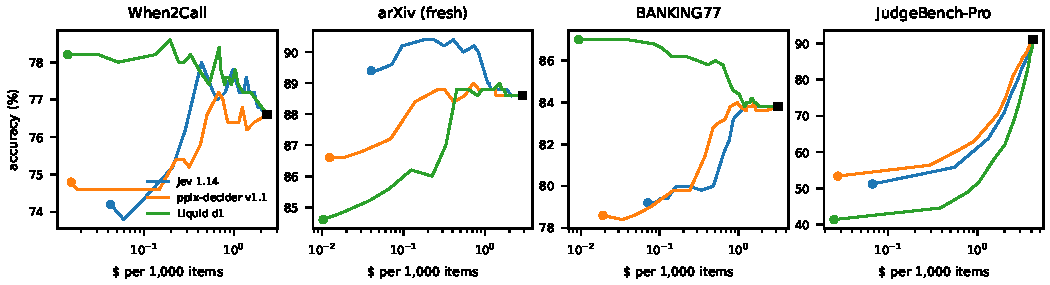
\includegraphics[width=\textwidth]{figures/cascade.pdf}
\caption{Cascades to GPT-6 Sol (E6): accuracy against cost as the threshold changes, for three System One models as the first stage, on all items (not cross-fitted). Circles: the System One model alone. Squares: GPT-6 Sol alone.}
\label{fig:cascade}
\end{figure*}

\begin{figure*}[t]
\centering
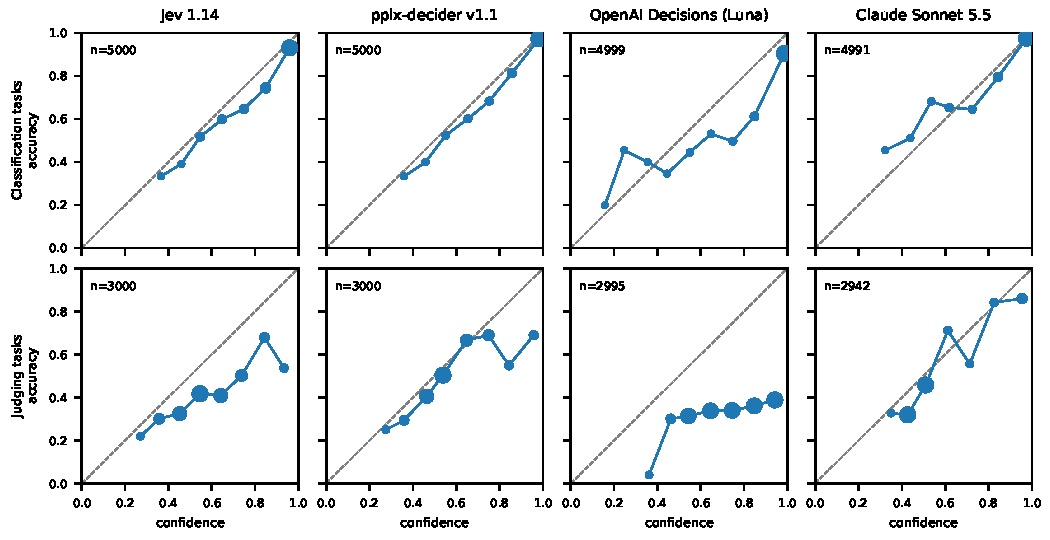
\includegraphics[width=\textwidth]{figures/reliability.pdf}
\caption{Reliability diagrams of the top answer (E2), with 10 equal-width bins (fewer bins than the ECE, so that each bin has enough answers). Points above the diagonal show underconfidence. Points below it show overconfidence. The size of a point shows the number of answers in the bin. The diagrams pool all questions of a group, so Civil Comments and HelpSteer2 weigh more.}
\label{fig:reliability}
\end{figure*}

\begin{table}[t]
\centering
\footnotesize
\setlength{\tabcolsep}{1.5pt}
\begin{tabular}{@{}lrrrrrr@{}}
\toprule
System & Calls & p50 & p95 & ms/1k & \$/1k & 7q/1q \\
\midrule
Jev 1.14 & 4000 & 514 & 621 & 8 & 0.042 & 0.99 \\
Jev 1.13 & 4000 & 513 & 606 & 11 & 0.042 & -- \\
OpenAI Decisions & 3994 & 295 & 420 & -14 & 0.085 & 0.94 \\
Microsoft-Decision-1 & 4000 & 544 & 666 & 1 & 0.026 & 1.08 \\
pplx-decider v1.1 & 4000 & 624 & 1152 & 94 & 0.021 & 1.78 \\
Clef & 4000 & 626 & 1158 & 56 & 0.222 & 1.00 \\
Clef-flash & 4000 & 541 & 1061 & 171 & 0.035 & 1.24 \\
Clef-omni & 4000 & 387 & 610 & 17 & 0.137 & 1.02 \\
Mercury Decide & 4000 & 602 & 809 & 93 & 0.017 & 1.09 \\
Kev-4B & 4000 & 853 & 1239 & 154 & 0.025 & 1.01 \\
Liquid d1 & 4000 & 637 & 841 & 20 & 0.017 & 1.06 \\
Drex v1.5 & 4000 & 546 & 1165 & 6 & 0.024 & 0.77 \\
Drex v2.0 & 4000 & 547 & 1116 & 9 & 0.036 & 0.98 \\
Span-01 & 1500 & 544 & 781 & -25 & 0.007 & 0.90 \\
Span-01-lite & 1500 & 547 & 788 & -69 & 0.000 & 0.90 \\
Classify-1 & 4000 & 1279 & 3672 & 108 & 0.067 & -- \\
Tev1-4B & 3484 & 548 & 1003 & 64 & 0.047 & 1.56 \\
Solar Decide & 3500 & 1256 & 18442 & 2565 & 0.088 & -- \\
Solar Decide Flash & 3500 & 751 & 1242 & 41 & 0.088 & 1.44 \\
GPT-6 Sol & 4000 & 2398 & 4240 & 1003 & 2.636 & -- \\
Claude Sonnet 5.5 & 3950 & 2241 & 4075 & 677 & 4.656 & -- \\
Gemini 3.8 Flash & 3998 & 3705 & 12773 & 937 & 1.663 & -- \\
Claude Haiku 5.5 & 3996 & 1904 & 5527 & 892 & 0.249 & -- \\
GPT-6 Luna (chat) & 4000 & 2984 & 6952 & 2097 & 0.164 & -- \\
\bottomrule
\end{tabular}
\caption{Latency and cost (E8, from the logs of E2 and B1). Times in ms, from Bangalore through OpenRouter, so they include the network. \emph{ms/1k}: the slope of the latency against the input tokens. \emph{\$/1k}: the cost of 1,000 calls. \emph{7q/1q}: Civil Comments, the median latency of one call with 7 questions divided by that of one call with 1 question.}
\label{tab:app-latency}
\end{table}


\end{document}
